%\renewcommand{\thesection}{\Alph{section}}
\renewcommand{\thechapter}{\Alph{chapter}}
\renewcommand{\thesection}{\Alph{chapter}.\arabic{section}}

%\addcontentsline{toc}{chapter}{Appendices}
%\chapter*{Appendices}
\appendixpage
%\newpage

% Saturation Tables
\newgeometry{margin=1.0 in}
\chapter{Steam Tables} \label{ch:appendixSteam}
Unless otherwise indicated, all data was sourced from the \href{https://webbook.nist.gov/chemistry/fluid/}{NIST Chemistry WebBook}, Accessed Dec. 2021.
\section{Saturation Properties for Steam - Temperature} \label{app:steam_satT}
\resetLTcolor
\begin{longtable}[!ht]{@{\zz\extracolsep{\fill}}cccccccccc}%{p{1cm}|p{1.5cm}|p{1.5cm}|p{1.5cm}|p{1.5cm}|p{1.5cm}|p{1.5cm}|p{1.5cm}|p{1.5cm}|p{1.5cm}}
%\begin{longtable}[!ht]{cccccccccc}%{p{1cm}|p{1.5cm}|p{1.5cm}|p{1.5cm}|p{1.5cm}|p{1.5cm}|p{1.5cm}|p{1.5cm}|p{1.5cm}|p{1.5cm}}
%    \centering
  %    \begin{tabular}{|l|l|l|l|l|l|l|l|l|l|}
  \multicolumn{1}{@{\fullwidthcolor{white}\extracolsep{\fill}}c}{\bf Temp.} & {\bf Pressure} & \multicolumn{2}{c}{\bf Spec. Volume} & \multicolumn{2}{c}{\bf Int. Energy} & \multicolumn{2}{c}{\bf Enthalpy} & \multicolumn{2}{c}{\bf Entropy} \\
  \multicolumn{1}{@{\fullwidthcolor{white}\extracolsep{\fill}}c}{$T$} & $p$  & $v_f$  & $v_g$  & $u_f$  & $u_g$  & $h_f$ & $h_g$  & $s_f$  & $s_g$  \\ %
  \multicolumn{1}{@{\fullwidthcolor{white}\extracolsep{\fill}}c}{°C} & MPa & $\rm m^3$/kg & $\rm m^3$/kg & kJ/kg & kJ/kg & kJ/kg & kJ/kg & kJ/kgK & kJ/kgK  \\ \hline\endhead 
  0.01 & 0.00061 & 0.00100 & 205.99 & 0 & 2374.9 & 0 & 2500.9 & 0.00 & 9.1555 \\ 
  5 & 0.00087 & 0.00100 & 147.01 & 21.019 & 2381.8 & 21.019 & 2510.1 & 0.0763 & 9.0248 \\ 
  10 & 0.00123 & 0.00100 & 106.3 & 42.020 & 2388.6 & 42.020 & 2519.2 & 0.1511 & 8.8998 \\ 
  15 & 0.00171 & 0.00100 & 77.875 & 62.980 & 2395.5 & 62.980 & 2528.3 & 0.2245 & 8.7803 \\ 
  20 & 0.00234 & 0.00100 & 57.757 & 83.912 & 2402.3 & 83.912 & 2537.4 & 0.2965 & 8.6660 \\ 
  25 & 0.00317 & 0.00100 & 43.337 & 104.83 & 2409.1 & 104.83 & 2546.5 & 0.3672 & 8.5566 \\ 
  30 & 0.00425 & 0.00100 & 32.878 & 125.73 & 2415.9 & 125.73 & 2555.5 & 0.4368 & 8.4520 \\ 
  35 & 0.00563 & 0.00101 & 25.205 & 146.63 & 2422.7 & 146.63 & 2564.5 & 0.5051 & 8.3517 \\ 
  40 & 0.00738 & 0.00101 & 19.515 & 167.53 & 2429.4 & 167.53 & 2573.5 & 0.5724 & 8.2555 \\ 
  45 & 0.00960 & 0.00101 & 15.252 & 188.43 & 2436.1 & 188.43 & 2582.4 & 0.6386 & 8.1633 \\ 
  50 & 0.01235 & 0.00101 & 12.027 & 209.33 & 2442.7 & 209.33 & 2591.3 & 0.7038 & 8.0748 \\ 
  55 & 0.01576 & 0.00101 & 9.5643 & 230.24 & 2449.3 & 230.24 & 2600.1 & 0.7680 & 7.9898 \\ 
  60 & 0.01995 & 0.00102 & 7.6672 & 251.16 & 2455.9 & 251.16 & 2608.8 & 0.8313 & 7.9081 \\ 
  65 & 0.02504 & 0.00102 & 6.1935 & 272.09 & 2462.4 & 272.09 & 2617.5 & 0.8937 & 7.8296 \\ 
  70 & 0.03120 & 0.00102 & 5.0395 & 293.03 & 2468.9 & 293.03 & 2626.1 & 0.9551 & 7.7540 \\ 
  75 & 0.03860 & 0.00103 & 4.1289 & 313.99 & 2475.2 & 313.99 & 2634.6 & 1.0158 & 7.6812 \\ 
  80 & 0.04741 & 0.00103 & 3.4052 & 334.96 & 2481.6 & 334.96 & 2643.0 & 1.0756 & 7.6111 \\ 
  85 & 0.05787 & 0.00103 & 2.8258 & 355.95 & 2487.8 & 355.95 & 2651.3 & 1.1346 & 7.5434 \\ 
  90 & 0.07018 & 0.00104 & 2.3591 & 376.97 & 2494.0 & 376.97 & 2659.5 & 1.1929 & 7.4781 \\ 
  95 & 0.08461 & 0.00104 & 1.9806 & 398.00 & 2500.0 & 398.00 & 2667.6 & 1.2504 & 7.4151 \\ 
  100 & 0.10142 & 0.00104 & 1.6718 & 419.06 & 2506.0 & 419.06 & 2675.6 & 1.3072 & 7.3541 \\ 
  105 & 0.12090 & 0.00105 & 1.4184 & 440.15 & 2511.9 & 440.15 & 2683.4 & 1.3633 & 7.2952 \\ 
  110 & 0.14338 & 0.00105 & 1.2093 & 461.26 & 2517.7 & 461.26 & 2691.1 & 1.4188 & 7.2381 \\ 
  115 & 0.16918 & 0.00106 & 1.0358 & 482.41 & 2523.3 & 482.41 & 2698.6 & 1.4737 & 7.1828 \\ 
  120 & 0.19867 & 0.00106 & 0.8912 & 503.60 & 2528.9 & 503.60 & 2705.9 & 1.5279 & 7.1291 \\ 
  125 & 0.23224 & 0.00106 & 0.7700 & 524.83 & 2534.3 & 524.83 & 2713.1 & 1.5816 & 7.0770 \\ 
  130 & 0.27028 & 0.00107 & 0.6680 & 546.09 & 2539.5 & 546.09 & 2720.1 & 1.6346 & 7.0264 \\ 
  135 & 0.31323 & 0.00107 & 0.5817 & 567.41 & 2544.7 & 567.41 & 2726.9 & 1.6872 & 6.9772 \\ 
  140 & 0.36154 & 0.00108 & 0.5085 & 588.77 & 2549.6 & 588.77 & 2733.4 & 1.7392 & 6.9293 \\ 
  145 & 0.41568 & 0.00109 & 0.4460 & 610.19 & 2554.4 & 610.19 & 2739.8 & 1.7907 & 6.8826 \\ 
  150 & 0.47616 & 0.00109 & 0.3925 & 631.66 & 2559.1 & 631.66 & 2745.9 & 1.8418 & 6.8371 \\ 
  155 & 0.54350 & 0.00110 & 0.3465 & 653.19 & 2563.5 & 653.19 & 2751.8 & 1.8924 & 6.7926 \\ 
  160 & 0.61823 & 0.00110 & 0.3068 & 674.79 & 2567.8 & 674.79 & 2757.4 & 1.9426 & 6.7491 \\ 
  165 & 0.70093 & 0.00111 & 0.2724 & 696.46 & 2571.9 & 696.46 & 2762.8 & 1.9923 & 6.7066 \\ 
  170 & 0.79219 & 0.00111 & 0.2426 & 718.20 & 2575.7 & 718.20 & 2767.9 & 2.0417 & 6.6650 \\ 
  175 & 0.8926 & 0.00112 & 0.2166 & 740.02 & 2579.4 & 740.02 & 2772.7 & 2.0906 & 6.6241 \\ 
  180 & 1.0028 & 0.00113 & 0.1938 & 761.92 & 2582.8 & 761.92 & 2777.2 & 2.1392 & 6.5840 \\ 
  185 & 1.1235 & 0.00113 & 0.1739 & 783.91 & 2586.0 & 783.91 & 2781.4 & 2.1875 & 6.5447 \\ 
  190 & 1.2552 & 0.00114 & 0.1564 & 806.00 & 2589.0 & 806.00 & 2785.3 & 2.2355 & 6.5059 \\ 
  195 & 1.3988 & 0.00115 & 0.1409 & 828.18 & 2591.7 & 828.18 & 2788.8 & 2.2832 & 6.4678 \\ 
  200 & 1.5549 & 0.00116 & 0.1272 & 850.47 & 2594.2 & 850.47 & 2792.0 & 2.3305 & 6.4302 \\ 
  205 & 1.7243 & 0.00116 & 0.1151 & 872.87 & 2596.4 & 872.87 & 2794.8 & 2.3777 & 6.3930 \\ 
  210 & 1.9077 & 0.00117 & 0.1043 & 895.39 & 2598.3 & 895.39 & 2797.3 & 2.4245 & 6.3563 \\ 
  215 & 2.1058 & 0.00118 & 0.0947 & 918.04 & 2599.9 & 918.04 & 2799.3 & 2.4712 & 6.3200 \\ 
  220 & 2.3196 & 0.00119 & 0.0861 & 940.82 & 2601.2 & 940.82 & 2800.9 & 2.5177 & 6.2840 \\ 
  225 & 2.5497 & 0.00120 & 0.0784 & 963.74 & 2602.2 & 963.74 & 2802.1 & 2.5640 & 6.2483 \\ 
  230 & 2.7971 & 0.00121 & 0.0715 & 986.81 & 2602.9 & 986.81 & 2802.9 & 2.6101 & 6.2128 \\ 
  235 & 3.0625 & 0.00122 & 0.0653 & 1010.0 & 2603.2 & 1010.0 & 2803.2 & 2.6561 & 6.1775 \\ 
  240 & 3.3469 & 0.00123 & 0.0597 & 1033.4 & 2603.1 & 1033.4 & 2803.0 & 2.7020 & 6.1423 \\ 
  245 & 3.6512 & 0.00124 & 0.0547 & 1057.0 & 2602.7 & 1057.0 & 2802.2 & 2.7478 & 6.1072 \\ 
  250 & 3.9762 & 0.00125 & 0.0501 & 1080.8 & 2601.8 & 1080.8 & 2800.9 & 2.7935 & 6.0721 \\ 
  255 & 4.3229 & 0.00126 & 0.0459 & 1104.8 & 2600.5 & 1104.8 & 2799.1 & 2.8392 & 6.0369 \\ 
  260 & 4.6923 & 0.00128 & 0.0422 & 1129.0 & 2598.7 & 1129.0 & 2796.6 & 2.8849 & 6.0016 \\ 
  265 & 5.0853 & 0.00129 & 0.0387 & 1153.4 & 2596.5 & 1153.4 & 2793.5 & 2.9307 & 5.9661 \\ 
  270 & 5.5030 & 0.00130 & 0.0356 & 1178.1 & 2593.7 & 1178.1 & 2789.7 & 2.9765 & 5.9304 \\ 
  275 & 5.9464 & 0.00132 & 0.0328 & 1203.1 & 2590.3 & 1203.1 & 2785.2 & 3.0224 & 5.8944 \\ 
  280 & 6.4166 & 0.00133 & 0.0302 & 1228.3 & 2586.4 & 1228.3 & 2779.9 & 3.0685 & 5.8579 \\ 
  285 & 6.9147 & 0.00135 & 0.0278 & 1253.9 & 2581.8 & 1253.9 & 2773.7 & 3.1147 & 5.8209 \\ 
  290 & 7.4418 & 0.00137 & 0.0256 & 1279.9 & 2576.5 & 1279.9 & 2766.7 & 3.1612 & 5.7834 \\ 
  295 & 7.9991 & 0.00138 & 0.0235 & 1306.2 & 2570.5 & 1306.2 & 2758.7 & 3.2080 & 5.7451 \\ 
  300 & 8.5879 & 0.00140 & 0.0217 & 1332.9 & 2563.6 & 1332.9 & 2749.6 & 3.2552 & 5.7059 \\ 
  305 & 9.2094 & 0.00143 & 0.0199 & 1360.2 & 2555.9 & 1360.2 & 2739.4 & 3.3028 & 5.6657 \\ 
  310 & 9.8651 & 0.00145 & 0.0183 & 1387.9 & 2547.1 & 1387.9 & 2727.9 & 3.3510 & 5.6244 \\ 
  315 & 10.556 & 0.00147 & 0.0169 & 1416.3 & 2537.2 & 1416.3 & 2715.1 & 3.3998 & 5.5816 \\ 
  320 & 11.284 & 0.00150 & 0.0155 & 1445.3 & 2526.0 & 1445.3 & 2700.6 & 3.4494 & 5.5372 \\ 
  325 & 12.051 & 0.00153 & 0.0142 & 1475.1 & 2513.4 & 1475.1 & 2684.3 & 3.5000 & 5.4908 \\ 
  330 & 12.858 & 0.00156 & 0.0130 & 1505.8 & 2499.2 & 1505.8 & 2666.0 & 3.5518 & 5.4422 \\ 
  335 & 13.707 & 0.00160 & 0.0118 & 1537.6 & 2483.0 & 1537.6 & 2645.4 & 3.6050 & 5.3906 \\ 
  340 & 14.601 & 0.00164 & 0.0108 & 1570.6 & 2464.4 & 1570.6 & 2621.8 & 3.6601 & 5.3356 \\ 
  345 & 15.541 & 0.00168 & 0.0098 & 1605.3 & 2443.1 & 1605.3 & 2594.9 & 3.7176 & 5.2762 \\ 
  350 & 16.529 & 0.00174 & 0.0088 & 1642.1 & 2418.1 & 1642.1 & 2563.6 & 3.7784 & 5.2110 \\ 
  355 & 17.570 & 0.00181 & 0.0079 & 1682.0 & 2388.4 & 1682.0 & 2526.6 & 3.8439 & 5.1380 \\ 
  360 & 18.666 & 0.00190 & 0.0069 & 1726.3 & 2351.8 & 1726.3 & 2481.5 & 3.9167 & 5.0536 \\ 
  365 & 19.821 & 0.00202 & 0.0060 & 1777.8 & 2303.8 & 1777.8 & 2422.9 & 4.0014 & 4.9497 \\ 
  370 & 21.044 & 0.00222 & 0.0050 & 1844.1 & 2230.3 & 1844.1 & 2334.5 & 4.1112 & 4.8012 \\ 
  373.9 & 22.052 & 0.00286 & 0.0034 & 1977.9 & 2058.6 & 1977.9 & 2133.5 & 4.3402 & 4.4831 \\ 

%    \end{tabular}
\end{longtable}
\newpage
\section{Saturation Properties for Steam - Pressure} \label{app:steam_satP}
\resetLTcolor

\begin{longtable}[!ht]{@{\zz\extracolsep{\fill}}cccccccccc}%{p{1cm}|p{1.5cm}|p{1.5cm}|p{1.5cm}|p{1.5cm}|p{1.5cm}|p{1.5cm}|p{1.5cm}|p{1.5cm}|p{1.5cm}}
%\begin{longtable}[!ht]{cccccccccc}%{p{1cm}|p{1.5cm}|p{1.5cm}|p{1.5cm}|p{1.5cm}|p{1.5cm}|p{1.5cm}|p{1.5cm}|p{1.5cm}|p{1.5cm}}
%    \centering
  %    \begin{tabular}{|l|l|l|l|l|l|l|l|l|l|}
  \multicolumn{1}{@{\fullwidthcolor{white}\extracolsep{\fill}}c}{\bf Pressure} & {\bf Temp.} & \multicolumn{2}{c}{\bf Spec. Volume} & \multicolumn{2}{c}{\bf Int. Energy} & \multicolumn{2}{c}{\bf Enthalpy} & \multicolumn{2}{c}{\bf Entropy} \\
  \multicolumn{1}{@{\fullwidthcolor{white}\extracolsep{\fill}}c}{$p$} & $T$  & $v_f$  & $v_g$  & $u_f$  & $u_g$  & $h_f$ & $h_g$  & $s_f$  & $s_g$  \\ %
  \multicolumn{1}{@{\fullwidthcolor{white}\extracolsep{\fill}}c}{MPa} & °C & $\rm m^3$/kg & $\rm m^3$/kg & kJ/kg & kJ/kg & kJ/kg & kJ/kg & kJ/kgK & kJ/kgK  \\ \hline\endhead 
        0.0010 & 6.970 & 0.00100 & 129.18 & 29.298 & 2384.5 & 29.299 & 2513.7 & 0.1059 & 8.9749 \\
        0.0012 & 9.654 & 0.00100 & 108.67 & 40.568 & 2388.2 & 40.569 & 2518.6 & 0.1460 & 8.9082 \\ 
        0.0014 & 11.969 & 0.00100 & 93.899 & 50.279 & 2391.3 & 50.280 & 2522.8 & 0.1802 & 8.8521 \\ 
        0.0016 & 14.010 & 0.00100 & 82.743 & 58.831 & 2394.1 & 58.833 & 2526.5 & 0.2100 & 8.8035 \\ 
%        0.0018 & 15.837 & 0.00100 & 74.011 & 66.487 & 2396.6 & 66.489 & 2529.9 & 0.2366 & 8.7608 \\ 
        0.002 & 17.495 & 0.00100 & 66.987 & 73.426 & 2398.9 & 73.428 & 2532.9 & 0.2606 & 8.7226 \\ 
        0.003 & 24.079 & 0.00100 & 45.653 & 100.97 & 2407.9 & 100.98 & 2544.8 & 0.3543 & 8.5764 \\ 
        0.004 & 28.960 & 0.00100 & 34.791 & 121.38 & 2414.5 & 121.39 & 2553.7 & 0.4224 & 8.4734 \\ 
        0.005 & 32.874 & 0.00101 & 28.185 & 137.74 & 2419.8 & 137.75 & 2560.7 & 0.4762 & 8.3938 \\ 
        0.006 & 36.159 & 0.00101 & 23.733 & 151.47 & 2424.2 & 151.48 & 2566.6 & 0.5208 & 8.3290 \\ 
        0.008 & 41.509 & 0.00101 & 18.099 & 173.83 & 2431.4 & 173.84 & 2576.2 & 0.5925 & 8.2273 \\ 
        0.010 & 45.806 & 0.00101 & 14.670 & 191.80 & 2437.2 & 191.81 & 2583.9 & 0.6492 & 8.1488 \\ 
        0.012 & 49.419 & 0.00101 & 12.358 & 206.90 & 2442.0 & 206.91 & 2590.3 & 0.6963 & 8.0849 \\ 
        0.014 & 52.547 & 0.00101 & 10.691 & 219.98 & 2446.1 & 219.99 & 2595.8 & 0.7366 & 8.0311 \\ 
        0.016 & 55.313 & 0.00101 & 9.4306 & 231.55 & 2449.8 & 231.57 & 2600.6 & 0.7720 & 7.9846 \\ 
%        0.018 & 57.798 & 0.00102 & 8.4431 & 241.95 & 2453.0 & 241.96 & 2605.0 & 0.8036 & 7.9437 \\ 
        0.02 & 60.058 & 0.00102 & 7.6480 & 251.40 & 2456.0 & 251.42 & 2608.9 & 0.8320 & 7.9072 \\ 
        0.03 & 69.095 & 0.00102 & 5.2284 & 289.24 & 2467.7 & 289.27 & 2624.5 & 0.9441 & 7.7675 \\ 
        0.04 & 75.857 & 0.00103 & 3.9930 & 317.58 & 2476.3 & 317.62 & 2636.1 & 1.0261 & 7.6690 \\ 
        0.05 & 81.317 & 0.00103 & 3.2400 & 340.49 & 2483.2 & 340.54 & 2645.2 & 1.0912 & 7.5930 \\ 
        0.06 & 85.926 & 0.00103 & 2.7317 & 359.84 & 2489.0 & 359.91 & 2652.9 & 1.1454 & 7.5311 \\ 
        0.08 & 93.486 & 0.00104 & 2.0871 & 391.63 & 2498.2 & 391.71 & 2665.2 & 1.2330 & 7.4339 \\ 
        0.10 & 99.606 & 0.00104 & 1.6939 & 417.40 & 2505.6 & 417.50 & 2674.9 & 1.3028 & 7.3588 \\ 
        0.12 & 104.78 & 0.00105 & 1.4284 & 439.23 & 2511.7 & 439.36 & 2683.1 & 1.3609 & 7.2977 \\ 
        0.14 & 109.29 & 0.00105 & 1.2366 & 458.27 & 2516.9 & 458.42 & 2690.0 & 1.4110 & 7.2461 \\ 
        0.16 & 113.30 & 0.00105 & 1.0914 & 475.21 & 2521.4 & 475.38 & 2696.0 & 1.4551 & 7.2014 \\ 
%        0.18 & 116.91 & 0.00106 & 0.97747 & 490.51 & 2525.5 & 490.70 & 2701.4 & 1.4945 & 7.1621 \\ 
        0.2 & 120.21 & 0.00106 & 0.88568 & 504.49 & 2529.1 & 504.70 & 2706.2 & 1.5302 & 7.1269 \\ 
        0.3 & 133.52 & 0.00107 & 0.60576 & 561.10 & 2543.2 & 561.43 & 2724.9 & 1.6717 & 6.9916 \\ 
        0.4 & 143.61 & 0.00108 & 0.46238 & 604.22 & 2553.1 & 604.65 & 2738.1 & 1.7765 & 6.8955 \\ 
        0.5 & 151.83 & 0.00109 & 0.37481 & 639.54 & 2560.7 & 640.09 & 2748.1 & 1.8604 & 6.8207 \\ 
        0.6 & 158.83 & 0.00110 & 0.31558 & 669.72 & 2566.8 & 670.38 & 2756.1 & 1.9308 & 6.7592 \\ 
        0.8 & 170.41 & 0.00111 & 0.24034 & 719.97 & 2576.0 & 720.86 & 2768.3 & 2.0457 & 6.6616 \\ 
        1.0 & 179.88 & 0.00113 & 0.19436 & 761.39 & 2582.7 & 762.52 & 2777.1 & 2.1381 & 6.5850 \\ 
        1.2 & 187.96 & 0.00114 & 0.16326 & 796.96 & 2587.8 & 798.33 & 2783.7 & 2.2159 & 6.5217 \\ 
        1.4 & 195.04 & 0.00115 & 0.14078 & 828.36 & 2591.8 & 829.97 & 2788.8 & 2.2835 & 6.4675 \\ 
        1.6 & 201.37 & 0.00116 & 0.12374 & 856.60 & 2594.8 & 858.46 & 2792.8 & 2.3435 & 6.4199 \\ 
%        1.8 & 207.11 & 0.00117 & 0.11037 & 882.37 & 2597.2 & 884.47 & 2795.9 & 2.3975 & 6.3775 \\ 
        2 & 212.38 & 0.00118 & 0.09959 & 906.14 & 2599.1 & 908.50 & 2798.3 & 2.4468 & 6.3390 \\ 
        3 & 233.85 & 0.00122 & 0.06666 & 1004.7 & 2603.2 & 1008.3 & 2803.2 & 2.6455 & 6.1856 \\ 
        4 & 250.35 & 0.00125 & 0.04978 & 1082.5 & 2601.7 & 1087.5 & 2800.8 & 2.7968 & 6.0696 \\ 
        5 & 263.94 & 0.00129 & 0.03945 & 1148.2 & 2597.0 & 1154.6 & 2794.2 & 2.9210 & 5.9737 \\ 
        6 & 275.58 & 0.00132 & 0.03245 & 1206.0 & 2589.9 & 1213.9 & 2784.6 & 3.0278 & 5.8901 \\ 
        8 & 295.01 & 0.00138 & 0.02353 & 1306.2 & 2570.5 & 1317.3 & 2758.7 & 3.2081 & 5.7450 \\ 
        10 & 311.00 & 0.00145 & 0.01803 & 1393.5 & 2545.2 & 1408.1 & 2725.5 & 3.3606 & 5.6160 \\ 
        12 & 324.68 & 0.00153 & 0.01426 & 1473.1 & 2514.3 & 1491.5 & 2685.4 & 3.4967 & 5.4939 \\ 
        14 & 336.67 & 0.00161 & 0.01149 & 1548.4 & 2477.1 & 1571.0 & 2637.9 & 3.6232 & 5.3727 \\ 
        16 & 347.35 & 0.00171 & 0.00931 & 1622.3 & 2431.8 & 1649.7 & 2580.8 & 3.7457 & 5.2463 \\ 
%        18 & 356.99 & 0.00184 & 0.00750 & 1699.0 & 2374.8 & 1732.1 & 2509.8 & 3.8718 & 5.1061 \\ 
        20 & 365.75 & 0.00204 & 0.00587 & 1786.4 & 2295.0 & 1827.2 & 2412.3 & 4.0156 & 4.9314 \\ 
        22 & 373.71 & 0.00270 & 0.00365 & 1951.8 & 2092.8 & 2011.3 & 2173.1 & 4.2945 & 4.5446 \\ 
        22.064 & 373.95 & 0.00311 & 0.00311 & 2015.7 & 2015.7 & 2084.3 & 2084.3 & 4.4070 & 4.4070 \\ 

%    \end{tabular}
\end{longtable}



% Superheated Tables
\newgeometry{margin=1.0in}
\section{Superheated Vapor Properties for Steam} \label{app:steam_super}
\resetLTcolor

% 10 kPa and 50 kPa
\begin{longtable}[!ht]{@{\zz\extracolsep{\fill}}c|cccc|cccc}
  \multicolumn{1}{@{\fullwidthcolor{white}\extracolsep{\fill}}c}{} & \multicolumn{4}{c|}{$p$ = 0.010 MPa ($T_{sat}$ = 45.8°C)} & \multicolumn{4}{c}{$p$ = 0.050 MPa ($T_{sat}$ = 81.3°C)} \\ \hline
  \multicolumn{1}{@{\fullwidthcolor{white}\extracolsep{\fill}}c|}{\bf Temp.} & {\bf Volume} & {\bf Energy} & {\bf Enthalpy} & {\bf Entropy}
  & {\bf Volume} & {\bf Energy} & {\bf Enthalpy} & {\bf Entropy} \\
  \multicolumn{1}{@{\fullwidthcolor{white}\extracolsep{\fill}}c|}{$T$} & $v$ & $u$ & $h$ & $s$ & $v$ & $u$ & $h$ & $s$ \\ %
  \multicolumn{1}{@{\fullwidthcolor{white}\extracolsep{\fill}}c|}{°C} & $\rm m^3$/kg & kJ/kg & kJ/kg & kJ/kgK & $\rm m^3$/kg & kJ/kg & kJ/kg & kJ/kgK \\ \hline\endhead 
          Sat. & 14.670 & 2437.2 & 2583.9 & 8.1488 & 3.2400 & 2483.2 & 2645.2 & 7.5930 \\ 
        50 & 14.867 & 2443.3 & 2592.0 & 8.1741 & ~ & ~ & ~ & ~ \\ 
        100 & 17.196 & 2515.5 & 2687.5 & 8.4489 & 3.4187 & 2511.5 & 2682.4 & 7.6953 \\ 
        150 & 19.513 & 2587.9 & 2783.0 & 8.6892 & 3.8897 & 2585.7 & 2780.2 & 7.9413 \\ 
        200 & 21.826 & 2661.3 & 2879.6 & 8.9049 & 4.3562 & 2660.0 & 2877.8 & 8.1592 \\ 
        250 & 24.136 & 2736.1 & 2977.4 & 9.1015 & 4.8206 & 2735.1 & 2976.1 & 8.3568 \\ 
        300 & 26.446 & 2812.3 & 3076.7 & 9.2827 & 5.2840 & 2811.6 & 3075.8 & 8.5386 \\ 
        350 & 28.755 & 2890.0 & 3177.5 & 9.4513 & 5.7469 & 2889.4 & 3176.8 & 8.7076 \\ 
        400 & 31.063 & 2969.3 & 3279.9 & 9.6094 & 6.2094 & 2968.9 & 3279.3 & 8.8659 \\ 
        450 & 33.371 & 3050.3 & 3384.0 & 9.7584 & 6.6717 & 3049.9 & 3383.5 & 9.0151 \\ 
        500 & 35.680 & 3132.9 & 3489.7 & 9.8998 & 7.1338 & 3132.6 & 3489.3 & 9.1566 \\ 
        550 & 37.988 & 3217.2 & 3597.1 & 10.034 & 7.5957 & 3217.0 & 3596.8 & 9.2913 \\ 
        600 & 40.296 & 3303.3 & 3706.3 & 10.163 & 8.0576 & 3303.1 & 3706.0 & 9.4201 \\ 
        650 & 42.603 & 3391.2 & 3817.2 & 10.287 & 8.5195 & 3391.0 & 3816.9 & 9.5436 \\ 
        700 & 44.911 & 3480.8 & 3929.9 & 10.406 & 8.9812 & 3480.6 & 3929.7 & 9.6625 \\ 
        750 & 47.219 & 3572.2 & 4044.4 & 10.520 & 9.4430 & 3572.0 & 4044.2 & 9.7773 \\ 
        800 & 49.527 & 3665.3 & 4160.6 & 10.631 & 9.9047 & 3665.2 & 4160.4 & 9.8882 \\ 
        850 & 51.835 & 3760.3 & 4278.6 & 10.739 & 10.366 & 3760.1 & 4278.5 & 9.9957 \\ 
        900 & 54.142 & 3856.9 & 4398.3 & 10.843 & 10.828 & 3856.8 & 4398.2 & 10.100 \\ 
        950 & 56.450 & 3955.2 & 4519.7 & 10.944 & 11.290 & 3955.1 & 4519.6 & 10.201 \\ 
        1000 & 58.758 & 4055.2 & 4642.8 & 11.043 & 11.751 & 4055.1 & 4642.7 & 10.300 

\end{longtable}

% 100 kPa and 200 kPa
\begin{longtable}[!ht]{@{\zz\extracolsep{\fill}}c|cccc|cccc}
  \multicolumn{1}{@{\fullwidthcolor{white}\extracolsep{\fill}}c}{} & \multicolumn{4}{c|}{$p$ = 0.10 MPa ($T_{sat}$ = 99.6°C)} & \multicolumn{4}{c}{$p$ = 0.20 MPa ($T_{sat}$ = 120.2°C)} \\ \hline
  \multicolumn{1}{@{\fullwidthcolor{white}\extracolsep{\fill}}c|}{\bf Temp.} & {\bf Volume} & {\bf Energy} & {\bf Enthalpy} & {\bf Entropy}
  & {\bf Volume} & {\bf Energy} & {\bf Enthalpy} & {\bf Entropy} \\
  \multicolumn{1}{@{\fullwidthcolor{white}\extracolsep{\fill}}c|}{$T$} & $v$ & $u$ & $h$ & $s$ & $v$ & $u$ & $h$ & $s$ \\ %
  \multicolumn{1}{@{\fullwidthcolor{white}\extracolsep{\fill}}c|}{°C} & $\rm m^3$/kg & kJ/kg & kJ/kg & kJ/kgK & $\rm m^3$/kg & kJ/kg & kJ/kg & kJ/kgK \\ \hline\endhead 
          Sat. & 1.6939 & 2505.6 & 2674.9 & 7.3588 & 0.8857 & 2529.1 & 2706.2 & 7.1269 \\ 
        100 & 1.6959 & 2506.2 & 2675.8 & 7.3610 & ~ & ~ & ~ & ~ \\ 
        150 & 1.9367 & 2582.9 & 2776.6 & 7.6148 & 0.9599 & 2577.1 & 2769.1 & 7.2810 \\ 
        200 & 2.1724 & 2658.2 & 2875.5 & 7.8356 & 1.0805 & 2654.6 & 2870.7 & 7.5081 \\ 
        250 & 2.4062 & 2733.9 & 2974.5 & 8.0346 & 1.1989 & 2731.4 & 2971.2 & 7.7100 \\ 
        300 & 2.6388 & 2810.6 & 3074.5 & 8.2172 & 1.3162 & 2808.8 & 3072.1 & 7.8941 \\ 
        350 & 2.8710 & 2888.7 & 3175.8 & 8.3866 & 1.4330 & 2887.3 & 3173.9 & 8.0644 \\ 
        400 & 3.1027 & 2968.3 & 3278.6 & 8.5452 & 1.5493 & 2967.1 & 3277.0 & 8.2236 \\ 
        450 & 3.3342 & 3049.4 & 3382.8 & 8.6946 & 1.6655 & 3048.5 & 3381.6 & 8.3734 \\ 
        500 & 3.5655 & 3132.2 & 3488.7 & 8.8361 & 1.7814 & 3131.4 & 3487.7 & 8.5152 \\ 
        550 & 3.7968 & 3216.6 & 3596.3 & 8.9709 & 1.8973 & 3215.9 & 3595.4 & 8.6502 \\ 
        600 & 4.0279 & 3302.8 & 3705.6 & 9.0998 & 2.0130 & 3302.2 & 3704.8 & 8.7792 \\ 
        650 & 4.2590 & 3390.7 & 3816.6 & 9.2234 & 2.1287 & 3390.2 & 3815.9 & 8.9030 \\ 
        700 & 4.4900 & 3480.4 & 3929.4 & 9.3424 & 2.2443 & 3479.9 & 3928.8 & 9.0220 \\ 
        750 & 4.7209 & 3571.8 & 4043.9 & 9.4572 & 2.3599 & 3571.4 & 4043.4 & 9.1369 \\ 
        800 & 4.9519 & 3665.0 & 4160.2 & 9.5681 & 2.4755 & 3664.7 & 4159.8 & 9.2479 \\ 
        850 & 5.1828 & 3760.0 & 4278.2 & 9.6757 & 2.5910 & 3759.6 & 4277.8 & 9.3555 \\ 
        900 & 5.4137 & 3856.6 & 4398.0 & 9.7800 & 2.7066 & 3856.3 & 4397.6 & 9.4598 \\ 
        950 & 5.6446 & 3955.0 & 4519.5 & 9.8813 & 2.8221 & 3954.7 & 4519.1 & 9.5612 \\ 
        1000 & 5.8754 & 4055.0 & 4642.6 & 9.9800 & 2.9375 & 4054.8 & 4642.3 & 9.6599

\end{longtable}


% 300 kPa and 400 kPa
\begin{longtable}[!ht]{@{\zz\extracolsep{\fill}}c|cccc|cccc}
  \multicolumn{1}{@{\fullwidthcolor{white}\extracolsep{\fill}}c}{} & \multicolumn{4}{c|}{$p$ = 0.30 MPa ($T_{sat}$ = 133.5°C)} & \multicolumn{4}{c}{$p$ = 0.40 MPa ($T_{sat}$ = 143.6°C)} \\ \hline
  \multicolumn{1}{@{\fullwidthcolor{white}\extracolsep{\fill}}c|}{\bf Temp.} & {\bf Volume} & {\bf Energy} & {\bf Enthalpy} & {\bf Entropy}
  & {\bf Volume} & {\bf Energy} & {\bf Enthalpy} & {\bf Entropy} \\
  \multicolumn{1}{@{\fullwidthcolor{white}\extracolsep{\fill}}c|}{$T$} & $v$ & $u$ & $h$ & $s$ & $v$ & $u$ & $h$ & $s$ \\ %
  \multicolumn{1}{@{\fullwidthcolor{white}\extracolsep{\fill}}c|}{°C} & $\rm m^3$/kg & kJ/kg & kJ/kg & kJ/kgK & $\rm m^3$/kg & kJ/kg & kJ/kg & kJ/kgK \\ \hline\endhead 
          Sat. & 0.6058 & 2543.2 & 2724.9 & 6.9916 & 0.4624 & 2553.1 & 2738.1 & 6.8955 \\ 
        150 & 0.6340 & 2571.0 & 2761.2 & 7.0791 & 0.4709 & 2564.4 & 2752.8 & 6.9306 \\ 
        200 & 0.7164 & 2651.0 & 2865.9 & 7.3131 & 0.5343 & 2647.2 & 2860.9 & 7.1723 \\ 
        250 & 0.7964 & 2728.9 & 2967.9 & 7.5180 & 0.5952 & 2726.4 & 2964.5 & 7.3804 \\ 
        300 & 0.8753 & 2807.0 & 3069.6 & 7.7037 & 0.6549 & 2805.1 & 3067.1 & 7.5677 \\ 
        350 & 0.9536 & 2885.9 & 3172.0 & 7.8750 & 0.7140 & 2884.4 & 3170.0 & 7.7399 \\ 
        400 & 1.0315 & 2966.0 & 3275.5 & 8.0347 & 0.7726 & 2964.9 & 3273.9 & 7.9002 \\ 
        450 & 1.1092 & 3047.5 & 3380.3 & 8.1849 & 0.8311 & 3046.6 & 3379.0 & 8.0508 \\ 
        500 & 1.1867 & 3130.6 & 3486.6 & 8.3271 & 0.8894 & 3129.8 & 3485.5 & 8.1933 \\ 
        550 & 1.2641 & 3215.3 & 3594.5 & 8.4623 & 0.9475 & 3214.6 & 3593.6 & 8.3287 \\ 
        600 & 1.3414 & 3301.6 & 3704.0 & 8.5914 & 1.0056 & 3301.0 & 3703.2 & 8.4580 \\ 
        650 & 1.4186 & 3389.7 & 3815.3 & 8.7153 & 1.0636 & 3389.1 & 3814.6 & 8.5820 \\ 
        700 & 1.4958 & 3479.5 & 3928.2 & 8.8344 & 1.1215 & 3479.0 & 3927.6 & 8.7012 \\ 
        750 & 1.5729 & 3571.0 & 4042.9 & 8.9494 & 1.1794 & 3570.6 & 4042.4 & 8.8162 \\ 
        800 & 1.6500 & 3664.3 & 4159.3 & 9.0604 & 1.2373 & 3663.9 & 4158.8 & 8.9273 \\ 
        850 & 1.7271 & 3759.3 & 4277.4 & 9.1680 & 1.2951 & 3759.0 & 4277.0 & 9.0350 \\ 
        900 & 1.8042 & 3856.0 & 4397.3 & 9.2724 & 1.3530 & 3855.7 & 4396.9 & 9.1394 \\ 
        950 & 1.8812 & 3954.4 & 4518.8 & 9.3739 & 1.4108 & 3954.2 & 4518.5 & 9.2409 \\ 
        1000 & 1.9582 & 4054.5 & 4642.0 & 9.4726 & 1.4686 & 4054.3 & 4641.7 & 9.3396 

\end{longtable}


% 500 kPa and 600 kPa
\begin{longtable}[!ht]{@{\zz\extracolsep{\fill}}c|cccc|cccc}
  \multicolumn{1}{@{\fullwidthcolor{white}\extracolsep{\fill}}c}{} & \multicolumn{4}{c|}{$p$ = 0.50 MPa ($T_{sat}$ = 151.8°C)} & \multicolumn{4}{c}{$p$ = 0.60 MPa ($T_{sat}$ = 158.8°C)} \\ \hline
  \multicolumn{1}{@{\fullwidthcolor{white}\extracolsep{\fill}}c|}{\bf Temp.} & {\bf Volume} & {\bf Energy} & {\bf Enthalpy} & {\bf Entropy}
  & {\bf Volume} & {\bf Energy} & {\bf Enthalpy} & {\bf Entropy} \\
  \multicolumn{1}{@{\fullwidthcolor{white}\extracolsep{\fill}}c|}{$T$} & $v$ & $u$ & $h$ & $s$ & $v$ & $u$ & $h$ & $s$ \\ %
  \multicolumn{1}{@{\fullwidthcolor{white}\extracolsep{\fill}}c|}{°C} & $\rm m^3$/kg & kJ/kg & kJ/kg & kJ/kgK & $\rm m^3$/kg & kJ/kg & kJ/kg & kJ/kgK \\ \hline\endhead 
          Sat. & 0.3748 & 2560.7 & 2748.1 & 6.8207 & 0.3156 & 2566.8 & 2756.1 & 6.7592 \\ 
        200 & 0.4250 & 2643.3 & 2855.8 & 7.0610 & 0.3521 & 2639.3 & 2850.6 & 6.9683 \\ 
        250 & 0.4744 & 2723.8 & 2961.0 & 7.2724 & 0.3939 & 2721.2 & 2957.6 & 7.1832 \\ 
        300 & 0.5226 & 2803.2 & 3064.6 & 7.4614 & 0.4344 & 2801.4 & 3062.0 & 7.3740 \\ 
        350 & 0.5702 & 2883.0 & 3168.1 & 7.6346 & 0.4743 & 2881.6 & 3166.1 & 7.5481 \\ 
        400 & 0.6173 & 2963.7 & 3272.3 & 7.7955 & 0.5137 & 2962.5 & 3270.8 & 7.7097 \\ 
        450 & 0.6642 & 3045.6 & 3377.7 & 7.9465 & 0.5530 & 3044.7 & 3376.5 & 7.8611 \\ 
        500 & 0.7109 & 3129.0 & 3484.5 & 8.0892 & 0.5920 & 3128.2 & 3483.4 & 8.0041 \\ 
        550 & 0.7576 & 3213.9 & 3592.7 & 8.2249 & 0.6309 & 3213.2 & 3591.8 & 8.1399 \\ 
        600 & 0.8041 & 3300.4 & 3702.5 & 8.3543 & 0.6698 & 3299.8 & 3701.7 & 8.2695 \\ 
        650 & 0.8506 & 3388.6 & 3813.9 & 8.4784 & 0.7085 & 3388.1 & 3813.2 & 8.3937 \\ 
        700 & 0.8970 & 3478.5 & 3927.0 & 8.5977 & 0.7473 & 3478.1 & 3926.4 & 8.5131 \\ 
        750 & 0.9433 & 3570.2 & 4041.8 & 8.7128 & 0.7859 & 3569.8 & 4041.3 & 8.6283 \\ 
        800 & 0.9897 & 3663.6 & 4158.4 & 8.8240 & 0.8246 & 3663.2 & 4157.9 & 8.7395 \\ 
        850 & 1.0360 & 3758.6 & 4276.6 & 8.9317 & 0.8632 & 3758.3 & 4276.2 & 8.8472 \\ 
        900 & 1.0823 & 3855.4 & 4396.6 & 9.0362 & 0.9018 & 3855.1 & 4396.2 & 8.9518 \\ 
        950 & 1.1285 & 3953.9 & 4518.2 & 9.1377 & 0.9404 & 3953.6 & 4517.8 & 9.0533 \\ 
        1000 & 1.1748 & 4054.0 & 4641.4 & 9.2364 & 0.9789 & 4053.7 & 4641.1 & 9.1521

\end{longtable}
\newpage
% 800 kPa and 1 MPa
\begin{longtable}[!ht]{@{\zz\extracolsep{\fill}}c|cccc|cccc}
  \multicolumn{1}{@{\fullwidthcolor{white}\extracolsep{\fill}}c}{} & \multicolumn{4}{c|}{$p$ = 0.80 MPa ($T_{sat}$ = 170.4°C)} & \multicolumn{4}{c}{$p$ = 1.0 MPa ($T_{sat}$ = 179.9°C)} \\ \hline
  \multicolumn{1}{@{\fullwidthcolor{white}\extracolsep{\fill}}c|}{\bf Temp.} & {\bf Volume} & {\bf Energy} & {\bf Enthalpy} & {\bf Entropy}
  & {\bf Volume} & {\bf Energy} & {\bf Enthalpy} & {\bf Entropy} \\
  \multicolumn{1}{@{\fullwidthcolor{white}\extracolsep{\fill}}c|}{$T$} & $v$ & $u$ & $h$ & $s$ & $v$ & $u$ & $h$ & $s$ \\ %
  \multicolumn{1}{@{\fullwidthcolor{white}\extracolsep{\fill}}c|}{°C} & $\rm m^3$/kg & kJ/kg & kJ/kg & kJ/kgK & $\rm m^3$/kg & kJ/kg & kJ/kg & kJ/kgK \\ \hline\endhead 
          Sat. & 0.2403 & 2576.0 & 2768.3 & 6.6616 & 0.1944 & 2582.7 & 2777.1 & 6.5850 \\ 
        200 & 0.2609 & 2631.0 & 2839.7 & 6.8176 & 0.2060 & 2622.2 & 2828.3 & 6.6955 \\ 
        250 & 0.2932 & 2715.9 & 2950.4 & 7.0401 & 0.2328 & 2710.4 & 2943.1 & 6.9265 \\ 
        300 & 0.3242 & 2797.5 & 3056.9 & 7.2345 & 0.2580 & 2793.6 & 3051.6 & 7.1246 \\ 
        350 & 0.3544 & 2878.6 & 3162.2 & 7.4106 & 0.2825 & 2875.7 & 3158.2 & 7.3029 \\ 
        400 & 0.3843 & 2960.2 & 3267.6 & 7.5734 & 0.3066 & 2957.9 & 3264.5 & 7.4669 \\ 
        450 & 0.4139 & 3042.8 & 3373.9 & 7.7257 & 0.3305 & 3040.9 & 3371.3 & 7.6200 \\ 
        500 & 0.4433 & 3126.6 & 3481.3 & 7.8692 & 0.3541 & 3125.0 & 3479.1 & 7.7641 \\ 
        550 & 0.4726 & 3211.9 & 3590.0 & 8.0054 & 0.3777 & 3210.5 & 3588.1 & 7.9008 \\ 
        600 & 0.5019 & 3298.7 & 3700.1 & 8.1354 & 0.4011 & 3297.5 & 3698.6 & 8.0310 \\ 
        650 & 0.5310 & 3387.1 & 3811.9 & 8.2598 & 0.4245 & 3386.0 & 3810.5 & 8.1557 \\ 
        700 & 0.5601 & 3477.2 & 3925.3 & 8.3794 & 0.4478 & 3476.2 & 3924.1 & 8.2755 \\ 
        750 & 0.5892 & 3569.0 & 4040.3 & 8.4947 & 0.4711 & 3568.1 & 4039.3 & 8.3909 \\ 
        800 & 0.6182 & 3662.4 & 4157.0 & 8.6061 & 0.4944 & 3661.7 & 4156.1 & 8.5024 \\ 
        850 & 0.6472 & 3757.6 & 4275.4 & 8.7139 & 0.5176 & 3757.0 & 4274.6 & 8.6103 \\ 
        900 & 0.6762 & 3854.5 & 4395.5 & 8.8185 & 0.5408 & 3853.9 & 4394.8 & 8.7150 \\ 
        950 & 0.7052 & 3953.1 & 4517.2 & 8.9201 & 0.5640 & 3952.5 & 4516.5 & 8.8166 \\ 
        1000 & 0.7341 & 4053.2 & 4640.5 & 9.0189 & 0.5872 & 4052.7 & 4639.9 & 8.9155  

\end{longtable}


% 1.2 MPa and 1.4 MPa
\begin{longtable}[!ht]{@{\zz\extracolsep{\fill}}c|cccc|cccc}
  \multicolumn{1}{@{\fullwidthcolor{white}\extracolsep{\fill}}c}{} & \multicolumn{4}{c|}{$p$ = 1.2 MPa ($T_{sat}$ = 188.0°C)} & \multicolumn{4}{c}{$p$ = 1.4 MPa ($T_{sat}$ = 195.0°C)} \\ \hline
  \multicolumn{1}{@{\fullwidthcolor{white}\extracolsep{\fill}}c|}{\bf Temp.} & {\bf Volume} & {\bf Energy} & {\bf Enthalpy} & {\bf Entropy}
  & {\bf Volume} & {\bf Energy} & {\bf Enthalpy} & {\bf Entropy} \\
  \multicolumn{1}{@{\fullwidthcolor{white}\extracolsep{\fill}}c|}{$T$} & $v$ & $u$ & $h$ & $s$ & $v$ & $u$ & $h$ & $s$ \\ %
  \multicolumn{1}{@{\fullwidthcolor{white}\extracolsep{\fill}}c|}{°C} & $\rm m^3$/kg & kJ/kg & kJ/kg & kJ/kgK & $\rm m^3$/kg & kJ/kg & kJ/kg & kJ/kgK \\ \hline\endhead 
  Sat. & 0.1633 & 2587.8 & 2783.7 & 6.5217 & 0.1408 & 2591.8 & 2788.8 & 6.4675 \\ 
        200 & 0.1693 & 2612.9 & 2816.1 & 6.5909 & 0.1430 & 2602.7 & 2803.0 & 6.4975 \\ 
        250 & 0.1924 & 2704.7 & 2935.6 & 6.8313 & 0.1636 & 2698.9 & 2927.9 & 6.7488 \\ 
        300 & 0.2139 & 2789.7 & 3046.3 & 7.0335 & 0.1823 & 2785.7 & 3040.9 & 6.9552 \\ 
        350 & 0.2346 & 2872.7 & 3154.2 & 7.2139 & 0.2003 & 2869.7 & 3150.1 & 7.1379 \\ 
        400 & 0.2548 & 2955.5 & 3261.3 & 7.3793 & 0.2178 & 2953.1 & 3258.1 & 7.3046 \\ 
        450 & 0.2748 & 3038.9 & 3368.7 & 7.5332 & 0.2351 & 3037.0 & 3366.1 & 7.4594 \\ 
        500 & 0.2946 & 3123.4 & 3476.9 & 7.6779 & 0.2522 & 3121.8 & 3474.8 & 7.6047 \\ 
        550 & 0.3143 & 3209.1 & 3586.3 & 7.8150 & 0.2691 & 3207.7 & 3584.5 & 7.7422 \\ 
        600 & 0.3339 & 3296.3 & 3697.0 & 7.9455 & 0.2860 & 3295.1 & 3695.4 & 7.8730 \\ 
        650 & 0.3535 & 3385.0 & 3809.2 & 8.0704 & 0.3028 & 3384.0 & 3807.8 & 7.9982 \\ 
        700 & 0.3730 & 3475.3 & 3922.9 & 8.1904 & 0.3195 & 3474.4 & 3921.7 & 8.1183 \\ 
        750 & 0.3924 & 3567.3 & 4038.2 & 8.3060 & 0.3362 & 3566.5 & 4037.2 & 8.2340 \\ 
        800 & 0.4118 & 3661.0 & 4155.2 & 8.4176 & 0.3529 & 3660.2 & 4154.3 & 8.3457 \\ 
        850 & 0.4312 & 3756.3 & 4273.8 & 8.5256 & 0.3695 & 3755.6 & 4273.0 & 8.4538 \\ 
        900 & 0.4506 & 3853.3 & 4394.0 & 8.6303 & 0.3861 & 3852.7 & 4393.3 & 8.5587 \\ 
        950 & 0.4699 & 3952.0 & 4515.9 & 8.7320 & 0.4027 & 3951.4 & 4515.2 & 8.6604 \\ 
        1000 & 0.4893 & 4052.2 & 4639.4 & 8.8310 & 0.4193 & 4051.7 & 4638.8 & 8.7594 

\end{longtable}
\newpage
% 1.6 MPa and 1.8 MPa
\begin{longtable}[!ht]{@{\zz\extracolsep{\fill}}c|cccc|cccc}
  \multicolumn{1}{@{\fullwidthcolor{white}\extracolsep{\fill}}c}{} & \multicolumn{4}{c|}{$p$ = 1.6 MPa ($T_{sat}$ = 201.4°C)} & \multicolumn{4}{c}{$p$ = 1.8 MPa ($T_{sat}$ = 207.1°C)} \\ \hline
  \multicolumn{1}{@{\fullwidthcolor{white}\extracolsep{\fill}}c|}{\bf Temp.} & {\bf Volume} & {\bf Energy} & {\bf Enthalpy} & {\bf Entropy}
  & {\bf Volume} & {\bf Energy} & {\bf Enthalpy} & {\bf Entropy} \\
  \multicolumn{1}{@{\fullwidthcolor{white}\extracolsep{\fill}}c|}{$T$} & $v$ & $u$ & $h$ & $s$ & $v$ & $u$ & $h$ & $s$ \\ %
  \multicolumn{1}{@{\fullwidthcolor{white}\extracolsep{\fill}}c|}{°C} & $\rm m^3$/kg & kJ/kg & kJ/kg & kJ/kgK & $\rm m^3$/kg & kJ/kg & kJ/kg & kJ/kgK \\ \hline\endhead 
          Sat. & 0.1237 & 2594.8 & 2792.8 & 6.4199 & 0.1104 & 2597.2 & 2795.9 & 6.3775 \\
        250 & 0.1419 & 2692.9 & 2919.9 & 6.6753 & 0.1250 & 2686.7 & 2911.7 & 6.6087 \\ 
        300 & 0.1587 & 2781.6 & 3035.4 & 6.8863 & 0.1403 & 2777.4 & 3029.9 & 6.8246 \\ 
        350 & 0.1746 & 2866.6 & 3146.0 & 7.0713 & 0.1546 & 2863.6 & 3141.8 & 7.0120 \\ 
        400 & 0.1901 & 2950.7 & 3254.9 & 7.2394 & 0.1685 & 2948.3 & 3251.6 & 7.1814 \\ 
        450 & 0.2053 & 3035.0 & 3363.5 & 7.3950 & 0.1821 & 3033.1 & 3360.9 & 7.3380 \\ 
        500 & 0.2203 & 3120.1 & 3472.6 & 7.5409 & 0.1955 & 3118.5 & 3470.4 & 7.4845 \\ 
        550 & 0.2352 & 3206.3 & 3582.6 & 7.6788 & 0.2088 & 3205.0 & 3580.8 & 7.6228 \\ 
        600 & 0.2500 & 3293.9 & 3693.9 & 7.8100 & 0.2220 & 3292.7 & 3692.3 & 7.7543 \\ 
        650 & 0.2647 & 3382.9 & 3806.5 & 7.9354 & 0.2351 & 3381.9 & 3805.1 & 7.8799 \\ 
        700 & 0.2794 & 3473.5 & 3920.5 & 8.0557 & 0.2482 & 3472.6 & 3919.4 & 8.0004 \\ 
        750 & 0.2940 & 3565.7 & 4036.1 & 8.1716 & 0.2613 & 3564.9 & 4035.1 & 8.1164 \\ 
        800 & 0.3087 & 3659.5 & 4153.3 & 8.2834 & 0.2743 & 3658.8 & 4152.4 & 8.2284 \\ 
        850 & 0.3232 & 3755.0 & 4272.2 & 8.3916 & 0.2872 & 3754.3 & 4271.3 & 8.3367 \\ 
        900 & 0.3378 & 3852.1 & 4392.6 & 8.4965 & 0.3002 & 3851.5 & 4391.9 & 8.4416 \\ 
        950 & 0.3523 & 3950.9 & 4514.6 & 8.5984 & 0.3131 & 3950.3 & 4514.0 & 8.5435 \\ 
        1000 & 0.3669 & 4051.2 & 4638.2 & 8.6974 & 0.3261 & 4050.7 & 4637.6 & 8.6426 

\end{longtable}

% 2.0 MPa and 2.5 MPa
\begin{longtable}[!ht]{@{\zz\extracolsep{\fill}}c|cccc|cccc}
  \multicolumn{1}{@{\fullwidthcolor{white}\extracolsep{\fill}}c}{} & \multicolumn{4}{c|}{$p$ = 2.0 MPa ($T_{sat}$ = 212.4°C)} & \multicolumn{4}{c}{$p$ = 2.5 MPa ($T_{sat}$ = 224.0°C)} \\ \hline
  \multicolumn{1}{@{\fullwidthcolor{white}\extracolsep{\fill}}c|}{\bf Temp.} & {\bf Volume} & {\bf Energy} & {\bf Enthalpy} & {\bf Entropy}
  & {\bf Volume} & {\bf Energy} & {\bf Enthalpy} & {\bf Entropy} \\
  \multicolumn{1}{@{\fullwidthcolor{white}\extracolsep{\fill}}c|}{$T$} & $v$ & $u$ & $h$ & $s$ & $v$ & $u$ & $h$ & $s$ \\ %
  \multicolumn{1}{@{\fullwidthcolor{white}\extracolsep{\fill}}c|}{°C} & $\rm m^3$/kg & kJ/kg & kJ/kg & kJ/kgK & $\rm m^3$/kg & kJ/kg & kJ/kg & kJ/kgK \\ \hline\endhead 
          Sat. & 0.0996 & 2599.1 & 2798.3 & 6.3390 & 0.0799 & 2602.1 & 2801.9 & 6.2558 \\
        250 & 0.1115 & 2680.2 & 2903.2 & 6.5475 & 0.0871 & 2663.3 & 2880.9 & 6.4107 \\ 
        300 & 0.1255 & 2773.2 & 3024.2 & 6.7684 & 0.0989 & 2762.2 & 3009.6 & 6.6459 \\ 
        350 & 0.1386 & 2860.5 & 3137.7 & 6.9583 & 0.1098 & 2852.5 & 3127.0 & 6.8424 \\ 
        400 & 0.1512 & 2945.9 & 3248.3 & 7.1292 & 0.1201 & 2939.8 & 3240.1 & 7.0170 \\ 
        450 & 0.1635 & 3031.1 & 3358.2 & 7.2866 & 0.1302 & 3026.2 & 3351.6 & 7.1767 \\ 
        500 & 0.1757 & 3116.9 & 3468.2 & 7.4337 & 0.1400 & 3112.8 & 3462.7 & 7.3254 \\ 
        550 & 0.1877 & 3203.6 & 3579.0 & 7.5725 & 0.1497 & 3200.1 & 3574.3 & 7.4653 \\ 
        600 & 0.1996 & 3291.5 & 3690.7 & 7.7043 & 0.1593 & 3288.5 & 3686.8 & 7.5979 \\ 
        650 & 0.2115 & 3380.8 & 3803.8 & 7.8302 & 0.1689 & 3378.2 & 3800.4 & 7.7243 \\ 
        700 & 0.2233 & 3471.6 & 3918.2 & 7.9509 & 0.1784 & 3469.3 & 3915.2 & 7.8455 \\ 
        750 & 0.2350 & 3564.0 & 4034.1 & 8.0670 & 0.1878 & 3562.0 & 4031.5 & 7.9620 \\ 
        800 & 0.2467 & 3658.0 & 4151.5 & 8.1790 & 0.1972 & 3656.2 & 4149.2 & 8.0743 \\ 
        850 & 0.2584 & 3753.6 & 4270.5 & 8.2874 & 0.2066 & 3752.0 & 4268.5 & 8.1830 \\ 
        900 & 0.2701 & 3850.9 & 4391.1 & 8.3925 & 0.2160 & 3849.4 & 4389.3 & 8.2882 \\ 
        950 & 0.2818 & 3949.8 & 4513.3 & 8.4945 & 0.2253 & 3948.4 & 4511.7 & 8.3904 \\ 
        1000 & 0.2934 & 4050.2 & 4637.0 & 8.5936 & 0.2347 & 4048.9 & 4635.6 & 8.4896 

\end{longtable}
\newpage
% 3.0 MPa and 3.5 MPa
\begin{longtable}[!ht]{@{\zz\extracolsep{\fill}}c|cccc|cccc}
  \multicolumn{1}{@{\fullwidthcolor{white}\extracolsep{\fill}}c}{} & \multicolumn{4}{c|}{$p$ = 3.0 MPa ($T_{sat}$ = 233.9°C)} & \multicolumn{4}{c}{$p$ = 3.5 MPa ($T_{sat}$ = 242.6°C)} \\ \hline
  \multicolumn{1}{@{\fullwidthcolor{white}\extracolsep{\fill}}c|}{\bf Temp.} & {\bf Volume} & {\bf Energy} & {\bf Enthalpy} & {\bf Entropy}
  & {\bf Volume} & {\bf Energy} & {\bf Enthalpy} & {\bf Entropy} \\
  \multicolumn{1}{@{\fullwidthcolor{white}\extracolsep{\fill}}c|}{$T$} & $v$ & $u$ & $h$ & $s$ & $v$ & $u$ & $h$ & $s$ \\ %
  \multicolumn{1}{@{\fullwidthcolor{white}\extracolsep{\fill}}c|}{°C} & $\rm m^3$/kg & kJ/kg & kJ/kg & kJ/kgK & $\rm m^3$/kg & kJ/kg & kJ/kg & kJ/kgK \\ \hline\endhead 
          Sat. & 0.0667 & 2603.2 & 2803.2 & 6.1856 & 0.0571 & 2602.9 & 2802.6 & 6.1243 \\
        250 & 0.0706 & 2644.7 & 2856.5 & 6.2893 & 0.0588 & 2624.0 & 2829.7 & 6.1764 \\ 
        300 & 0.0812 & 2750.8 & 2994.3 & 6.5412 & 0.0685 & 2738.8 & 2978.4 & 6.4484 \\ 
        350 & 0.0906 & 2844.4 & 3116.1 & 6.7449 & 0.0768 & 2836.0 & 3104.8 & 6.6601 \\ 
        400 & 0.0994 & 2933.5 & 3231.7 & 6.9234 & 0.0846 & 2927.2 & 3223.2 & 6.8427 \\ 
        450 & 0.1079 & 3021.2 & 3344.8 & 7.0856 & 0.0920 & 3016.1 & 3338.0 & 7.0074 \\ 
        500 & 0.1162 & 3108.6 & 3457.2 & 7.2359 & 0.0992 & 3104.5 & 3451.6 & 7.1593 \\ 
        550 & 0.1244 & 3196.6 & 3569.7 & 7.3768 & 0.1063 & 3193.1 & 3565.0 & 7.3014 \\ 
        600 & 0.1325 & 3285.5 & 3682.8 & 7.5103 & 0.1133 & 3282.5 & 3678.9 & 7.4356 \\ 
        650 & 0.1405 & 3375.6 & 3796.9 & 7.6373 & 0.1202 & 3372.9 & 3793.5 & 7.5633 \\ 
        700 & 0.1484 & 3467.0 & 3912.2 & 7.7590 & 0.1270 & 3464.7 & 3909.3 & 7.6854 \\ 
        750 & 0.1563 & 3559.9 & 4028.9 & 7.8758 & 0.1338 & 3557.8 & 4026.3 & 7.8027 \\ 
        800 & 0.1642 & 3654.3 & 4146.9 & 7.9885 & 0.1406 & 3652.5 & 4144.6 & 7.9156 \\ 
        850 & 0.1721 & 3750.3 & 4266.5 & 8.0973 & 0.1474 & 3748.6 & 4264.4 & 8.0247 \\ 
        900 & 0.1799 & 3847.9 & 4387.5 & 8.2028 & 0.1541 & 3846.4 & 4385.7 & 8.1303 \\ 
        950 & 0.1877 & 3947.0 & 4510.1 & 8.3051 & 0.1608 & 3945.6 & 4508.4 & 8.2328 \\ 
        1000 & 0.1955 & 4047.7 & 4634.1 & 8.4045 & 0.1675 & 4046.4 & 4632.7 & 8.3324 

\end{longtable}

% 4.0 MPa and 4.5 MPa
\begin{longtable}[!ht]{@{\zz\extracolsep{\fill}}c|cccc|cccc}
  \multicolumn{1}{@{\fullwidthcolor{white}\extracolsep{\fill}}c}{} & \multicolumn{4}{c|}{$p$ = 4.0 MPa ($T_{sat}$ = 250.4°C)} & \multicolumn{4}{c}{$p$ = 4.5 MPa ($T_{sat}$ = 257.4°C)} \\ \hline
  \multicolumn{1}{@{\fullwidthcolor{white}\extracolsep{\fill}}c|}{\bf Temp.} & {\bf Volume} & {\bf Energy} & {\bf Enthalpy} & {\bf Entropy}
  & {\bf Volume} & {\bf Energy} & {\bf Enthalpy} & {\bf Entropy} \\
  \multicolumn{1}{@{\fullwidthcolor{white}\extracolsep{\fill}}c|}{$T$} & $v$ & $u$ & $h$ & $s$ & $v$ & $u$ & $h$ & $s$ \\ %
  \multicolumn{1}{@{\fullwidthcolor{white}\extracolsep{\fill}}c|}{°C} & $\rm m^3$/kg & kJ/kg & kJ/kg & kJ/kgK & $\rm m^3$/kg & kJ/kg & kJ/kg & kJ/kgK \\ \hline\endhead 
          Sat. & 0.0498 & 2601.7 & 2800.8 & 6.0696 & 0.0441 & 2599.7 & 2797.9 & 6.0197 \\
        300 & 0.0589 & 2726.2 & 2961.7 & 6.3639 & 0.0514 & 2713.0 & 2944.2 & 6.2854 \\ 
        350 & 0.0665 & 2827.4 & 3093.3 & 6.5843 & 0.0584 & 2818.6 & 3081.5 & 6.5153 \\ 
        400 & 0.0734 & 2920.7 & 3214.5 & 6.7714 & 0.0648 & 2914.2 & 3205.6 & 6.7070 \\ 
        450 & 0.0800 & 3011.0 & 3331.2 & 6.9386 & 0.0708 & 3005.8 & 3324.2 & 6.8770 \\ 
        500 & 0.0864 & 3100.3 & 3446.0 & 7.0922 & 0.0765 & 3096.0 & 3440.4 & 7.0323 \\ 
        550 & 0.0927 & 3189.5 & 3560.3 & 7.2355 & 0.0821 & 3186.0 & 3555.6 & 7.1767 \\ 
        600 & 0.0989 & 3279.4 & 3674.9 & 7.3705 & 0.0877 & 3276.4 & 3670.9 & 7.3127 \\ 
        650 & 0.1049 & 3370.3 & 3790.1 & 7.4988 & 0.0931 & 3367.7 & 3786.6 & 7.4416 \\ 
        700 & 0.1110 & 3462.4 & 3906.3 & 7.6214 & 0.0985 & 3460.0 & 3903.3 & 7.5646 \\ 
        750 & 0.1170 & 3555.8 & 4023.6 & 7.7390 & 0.1039 & 3553.7 & 4021.0 & 7.6826 \\ 
        800 & 0.1229 & 3650.6 & 4142.3 & 7.8523 & 0.1092 & 3648.8 & 4140.0 & 7.7962 \\ 
        850 & 0.1289 & 3747.0 & 4262.4 & 7.9616 & 0.1145 & 3745.3 & 4260.3 & 7.9057 \\ 
        900 & 0.1348 & 3844.8 & 4383.9 & 8.0674 & 0.1197 & 3843.3 & 4382.1 & 8.0118 \\ 
        950 & 0.1407 & 3944.2 & 4506.8 & 8.1701 & 0.1250 & 3942.8 & 4505.2 & 8.1146 \\ 
        1000 & 0.1465 & 4045.1 & 4631.2 & 8.2697 & 0.1302 & 4043.9 & 4629.8 & 8.2144 

\end{longtable}
\newpage
% 5 MPa and 6 MPa
\begin{longtable}[!ht]{@{\zz\extracolsep{\fill}}c|cccc|cccc}
  \multicolumn{1}{@{\fullwidthcolor{white}\extracolsep{\fill}}c}{} & \multicolumn{4}{c|}{$p$ = 5.0 MPa ($T_{sat}$ = 263.9°C)} & \multicolumn{4}{c}{$p$ = 6.0 MPa ($T_{sat}$ = 275.6°C)} \\ \hline
  \multicolumn{1}{@{\fullwidthcolor{white}\extracolsep{\fill}}c|}{\bf Temp.} & {\bf Volume} & {\bf Energy} & {\bf Enthalpy} & {\bf Entropy}
  & {\bf Volume} & {\bf Energy} & {\bf Enthalpy} & {\bf Entropy} \\
  \multicolumn{1}{@{\fullwidthcolor{white}\extracolsep{\fill}}c|}{$T$} & $v$ & $u$ & $h$ & $s$ & $v$ & $u$ & $h$ & $s$ \\ %
  \multicolumn{1}{@{\fullwidthcolor{white}\extracolsep{\fill}}c|}{°C} & $\rm m^3$/kg & kJ/kg & kJ/kg & kJ/kgK & $\rm m^3$/kg & kJ/kg & kJ/kg & kJ/kgK \\ \hline\endhead 
          Sat. & 0.0394 & 2597.0 & 2794.2 & 5.9737 & 0.0324 & 2589.9 & 2784.6 & 5.8901 \\
        300 & 0.0453 & 2699.0 & 2925.7 & 6.2110 & 0.0362 & 2668.4 & 2885.5 & 6.0703 \\ 
        350 & 0.0520 & 2809.5 & 3069.3 & 6.4516 & 0.0423 & 2790.4 & 3043.9 & 6.3357 \\ 
        400 & 0.0578 & 2907.5 & 3196.7 & 6.6483 & 0.0474 & 2893.7 & 3178.2 & 6.5432 \\ 
        450 & 0.0633 & 3000.6 & 3317.2 & 6.8210 & 0.0522 & 2989.9 & 3302.9 & 6.7219 \\ 
        500 & 0.0686 & 3091.7 & 3434.7 & 6.9781 & 0.0567 & 3083.1 & 3423.1 & 6.8826 \\ 
        550 & 0.0737 & 3182.4 & 3550.9 & 7.1237 & 0.0610 & 3175.2 & 3541.3 & 7.0307 \\ 
        600 & 0.0787 & 3273.3 & 3666.8 & 7.2605 & 0.0653 & 3267.2 & 3658.7 & 7.1693 \\ 
        650 & 0.0836 & 3365.0 & 3783.2 & 7.3901 & 0.0694 & 3359.6 & 3776.2 & 7.3001 \\ 
        700 & 0.0885 & 3457.7 & 3900.3 & 7.5136 & 0.0735 & 3453.0 & 3894.3 & 7.4246 \\ 
        750 & 0.0934 & 3551.6 & 4018.4 & 7.6320 & 0.0776 & 3547.5 & 4013.2 & 7.5438 \\ 
        800 & 0.0982 & 3646.9 & 4137.7 & 7.7458 & 0.0816 & 3643.2 & 4133.1 & 7.6582 \\ 
        850 & 0.1029 & 3743.6 & 4258.3 & 7.8556 & 0.0857 & 3740.3 & 4254.2 & 7.7685 \\ 
        900 & 0.1077 & 3841.8 & 4380.2 & 7.9618 & 0.0896 & 3838.8 & 4376.6 & 7.8751 \\ 
        950 & 0.1124 & 3941.5 & 4503.6 & 8.0648 & 0.0936 & 3938.7 & 4500.3 & 7.9784 \\ 
        1000 & 0.1172 & 4042.6 & 4628.3 & 8.1648 & 0.0976 & 4040.1 & 4625.4 & 8.0786 

\end{longtable}

% 7 MPa and 8 MPa
\begin{longtable}[!ht]{@{\zz\extracolsep{\fill}}c|cccc|cccc}
  \multicolumn{1}{@{\fullwidthcolor{white}\extracolsep{\fill}}c}{} & \multicolumn{4}{c|}{$p$ = 7.0 MPa ($T_{sat}$ = 285.8°C)} & \multicolumn{4}{c}{$p$ = 8.0 MPa ($T_{sat}$ = 295.0°C)} \\ \hline
  \multicolumn{1}{@{\fullwidthcolor{white}\extracolsep{\fill}}c|}{\bf Temp.} & {\bf Volume} & {\bf Energy} & {\bf Enthalpy} & {\bf Entropy}
  & {\bf Volume} & {\bf Energy} & {\bf Enthalpy} & {\bf Entropy} \\
  \multicolumn{1}{@{\fullwidthcolor{white}\extracolsep{\fill}}c|}{$T$} & $v$ & $u$ & $h$ & $s$ & $v$ & $u$ & $h$ & $s$ \\ %
  \multicolumn{1}{@{\fullwidthcolor{white}\extracolsep{\fill}}c|}{°C} & $\rm m^3$/kg & kJ/kg & kJ/kg & kJ/kgK & $\rm m^3$/kg & kJ/kg & kJ/kg & kJ/kgK \\ \hline\endhead 
          Sat. & 0.0274 & 2581.0 & 2772.6 & 5.8148 & 0.0235 & 2570.5 & 2758.7 & 5.7450 \\
        300 & 0.0295 & 2633.5 & 2839.9 & 5.9337 & 0.0243 & 2592.3 & 2786.5 & 5.7937 \\ 
        350 & 0.0353 & 2770.1 & 3016.9 & 6.2304 & 0.0300 & 2748.3 & 2988.1 & 6.1321 \\ 
        400 & 0.0400 & 2879.5 & 3159.2 & 6.4502 & 0.0343 & 2864.6 & 3139.4 & 6.3658 \\ 
        450 & 0.0442 & 2979.0 & 3288.3 & 6.6353 & 0.0382 & 2967.8 & 3273.3 & 6.5579 \\ 
        500 & 0.0482 & 3074.3 & 3411.4 & 6.8000 & 0.0418 & 3065.4 & 3399.5 & 6.7266 \\ 
        550 & 0.0520 & 3167.9 & 3531.6 & 6.9506 & 0.0452 & 3160.5 & 3521.8 & 6.8799 \\ 
        600 & 0.0557 & 3260.9 & 3650.6 & 7.0910 & 0.0485 & 3254.7 & 3642.4 & 7.0221 \\ 
        650 & 0.0593 & 3354.3 & 3769.3 & 7.2231 & 0.0517 & 3348.9 & 3762.3 & 7.1556 \\ 
        700 & 0.0629 & 3448.3 & 3888.2 & 7.3486 & 0.0548 & 3443.6 & 3882.2 & 7.2821 \\ 
        750 & 0.0664 & 3543.3 & 4007.9 & 7.4685 & 0.0579 & 3539.1 & 4002.6 & 7.4028 \\ 
        800 & 0.0699 & 3639.5 & 4128.4 & 7.5836 & 0.0610 & 3635.7 & 4123.8 & 7.5184 \\ 
        850 & 0.0733 & 3736.9 & 4250.1 & 7.6944 & 0.0641 & 3733.5 & 4246.0 & 7.6297 \\ 
        900 & 0.0768 & 3835.7 & 4373.0 & 7.8014 & 0.0671 & 3832.6 & 4369.3 & 7.7371 \\ 
        950 & 0.0802 & 3935.9 & 4497.1 & 7.9050 & 0.0701 & 3933.1 & 4493.8 & 7.8411 \\ 
        1000 & 0.0836 & 4037.5 & 4622.5 & 8.0055 & 0.0731 & 4035.0 & 4619.6 & 7.9419 

\end{longtable}
\newpage
% 9 MPa and 10 MPa
\begin{longtable}[!ht]{@{\zz\extracolsep{\fill}}c|cccc|cccc}
  \multicolumn{1}{@{\fullwidthcolor{white}\extracolsep{\fill}}c}{} & \multicolumn{4}{c|}{$p$ = 9.0 MPa ($T_{sat}$ = 303.3°C)} & \multicolumn{4}{c}{$p$ = 10.0 MPa ($T_{sat}$ = 311.0°C)} \\ \hline
  \multicolumn{1}{@{\fullwidthcolor{white}\extracolsep{\fill}}c|}{\bf Temp.} & {\bf Volume} & {\bf Energy} & {\bf Enthalpy} & {\bf Entropy}
  & {\bf Volume} & {\bf Energy} & {\bf Enthalpy} & {\bf Entropy} \\
  \multicolumn{1}{@{\fullwidthcolor{white}\extracolsep{\fill}}c|}{$T$} & $v$ & $u$ & $h$ & $s$ & $v$ & $u$ & $h$ & $s$ \\ %
  \multicolumn{1}{@{\fullwidthcolor{white}\extracolsep{\fill}}c|}{°C} & $\rm m^3$/kg & kJ/kg & kJ/kg & kJ/kgK & $\rm m^3$/kg & kJ/kg & kJ/kg & kJ/kgK \\ \hline\endhead 
          Sat. & 0.0205 & 2558.5 & 2742.9 & 5.6791 & 0.0180 & 2545.2 & 2725.5 & 5.6160 \\
        350 & 0.0258 & 2724.9 & 2957.3 & 6.0380 & 0.0224 & 2699.6 & 2924.0 & 5.9459 \\ 
        400 & 0.0300 & 2849.2 & 3118.8 & 6.2876 & 0.0264 & 2833.1 & 3097.4 & 6.2141 \\ 
        450 & 0.0335 & 2956.3 & 3258.0 & 6.4872 & 0.0298 & 2944.5 & 3242.3 & 6.4219 \\ 
        500 & 0.0368 & 3056.3 & 3387.4 & 6.6603 & 0.0328 & 3047.0 & 3375.1 & 6.5995 \\ 
        550 & 0.0399 & 3153.0 & 3512.0 & 6.8164 & 0.0357 & 3145.4 & 3502.0 & 6.7585 \\ 
        600 & 0.0429 & 3248.4 & 3634.1 & 6.9605 & 0.0384 & 3242.0 & 3625.8 & 6.9045 \\ 
        650 & 0.0458 & 3343.4 & 3755.2 & 7.0953 & 0.0410 & 3337.9 & 3748.1 & 7.0408 \\ 
        700 & 0.0486 & 3438.8 & 3876.1 & 7.2229 & 0.0436 & 3434.0 & 3870.0 & 7.1693 \\ 
        750 & 0.0514 & 3534.9 & 3997.3 & 7.3443 & 0.0461 & 3530.7 & 3992.0 & 7.2916 \\ 
        800 & 0.0541 & 3632.0 & 4119.1 & 7.4606 & 0.0486 & 3628.2 & 4114.5 & 7.4085 \\ 
        850 & 0.0569 & 3730.2 & 4241.9 & 7.5724 & 0.0511 & 3726.8 & 4237.8 & 7.5207 \\ 
        900 & 0.0596 & 3829.6 & 4365.7 & 7.6802 & 0.0535 & 3826.5 & 4362.0 & 7.6290 \\ 
        950 & 0.0622 & 3930.3 & 4490.6 & 7.7844 & 0.0560 & 3927.5 & 4487.3 & 7.7335 \\ 
        1000 & 0.0649 & 4032.4 & 4616.7 & 7.8855 & 0.0584 & 4029.9 & 4613.8 & 7.8349 

\end{longtable}

% 12.5 MPa and 15 MPa
\begin{longtable}[!ht]{@{\zz\extracolsep{\fill}}c|cccc|cccc}
  \multicolumn{1}{@{\fullwidthcolor{white}\extracolsep{\fill}}c}{} & \multicolumn{4}{c|}{$p$ = 12.5 MPa ($T_{sat}$ = 327.8°C)} & \multicolumn{4}{c}{$p$ = 15.0 MPa ($T_{sat}$ = 342.16°C)} \\ \hline
  \multicolumn{1}{@{\fullwidthcolor{white}\extracolsep{\fill}}c|}{\bf Temp.} & {\bf Volume} & {\bf Energy} & {\bf Enthalpy} & {\bf Entropy}
  & {\bf Volume} & {\bf Energy} & {\bf Enthalpy} & {\bf Entropy} \\
  \multicolumn{1}{@{\fullwidthcolor{white}\extracolsep{\fill}}c|}{$T$} & $v$ & $u$ & $h$ & $s$ & $v$ & $u$ & $h$ & $s$ \\ %
  \multicolumn{1}{@{\fullwidthcolor{white}\extracolsep{\fill}}c|}{°C} & $\rm m^3$/kg & kJ/kg & kJ/kg & kJ/kgK & $\rm m^3$/kg & kJ/kg & kJ/kg & kJ/kgK \\ \hline\endhead 
          Sat. & 0.0135 & 2505.6 & 2674.3 & 5.4638 & 0.0103 & 2455.6 & 2610.7 & 5.3106 \\
        350 & 0.0161 & 2624.8 & 2826.6 & 5.7130 & 0.0115 & 2520.9 & 2693.1 & 5.4437 \\ 
        400 & 0.0200 & 2789.6 & 3040.0 & 6.0433 & 0.0157 & 2740.6 & 2975.7 & 5.8819 \\ 
        450 & 0.0230 & 2913.7 & 3201.4 & 6.2749 & 0.0185 & 2880.7 & 3157.9 & 6.1434 \\ 
        500 & 0.0256 & 3023.2 & 3343.6 & 6.4650 & 0.0208 & 2998.4 & 3310.8 & 6.3480 \\ 
        550 & 0.0280 & 3126.1 & 3476.5 & 6.6317 & 0.0229 & 3106.2 & 3450.4 & 6.5230 \\ 
        600 & 0.0303 & 3225.8 & 3604.6 & 6.7828 & 0.0249 & 3209.3 & 3583.1 & 6.6796 \\ 
        650 & 0.0325 & 3324.1 & 3730.2 & 6.9227 & 0.0268 & 3310.1 & 3712.1 & 6.8233 \\ 
        700 & 0.0346 & 3422.0 & 3854.6 & 7.0539 & 0.0286 & 3409.8 & 3839.1 & 6.9572 \\ 
        750 & 0.0367 & 3520.1 & 3978.6 & 7.1782 & 0.0304 & 3509.4 & 3965.2 & 7.0836 \\ 
        800 & 0.0387 & 3618.7 & 4102.8 & 7.2967 & 0.0321 & 3609.2 & 4091.1 & 7.2037 \\ 
        850 & 0.0407 & 3718.3 & 4227.5 & 7.4102 & 0.0338 & 3709.8 & 4217.1 & 7.3185 \\ 
        900 & 0.0427 & 3818.9 & 4352.9 & 7.5194 & 0.0355 & 3811.2 & 4343.7 & 7.4288 \\ 
        950 & 0.0447 & 3920.6 & 4479.2 & 7.6249 & 0.0372 & 3913.6 & 4471.0 & 7.5350 \\ 
        1000 & 0.0466 & 4023.5 & 4606.5 & 7.7269 & 0.0388 & 4017.1 & 4599.2 & 7.6378 

\end{longtable}
\newpage
% 17.5 MPa and 20 MPa
\begin{longtable}[!ht]{@{\zz\extracolsep{\fill}}c|cccc|cccc}
  \multicolumn{1}{@{\fullwidthcolor{white}\extracolsep{\fill}}c}{} & \multicolumn{4}{c|}{$p$ = 17.5 MPa ($T_{sat}$ = 354.7°C)} & \multicolumn{4}{c}{$p$ = 20.0 MPa ($T_{sat}$ = 365.8°C)} \\ \hline
  \multicolumn{1}{@{\fullwidthcolor{white}\extracolsep{\fill}}c|}{\bf Temp.} & {\bf Volume} & {\bf Energy} & {\bf Enthalpy} & {\bf Entropy}
  & {\bf Volume} & {\bf Energy} & {\bf Enthalpy} & {\bf Entropy} \\
  \multicolumn{1}{@{\fullwidthcolor{white}\extracolsep{\fill}}c|}{$T$} & $v$ & $u$ & $h$ & $s$ & $v$ & $u$ & $h$ & $s$ \\ %
  \multicolumn{1}{@{\fullwidthcolor{white}\extracolsep{\fill}}c|}{°C} & $\rm m^3$/kg & kJ/kg & kJ/kg & kJ/kgK & $\rm m^3$/kg & kJ/kg & kJ/kg & kJ/kgK \\ \hline\endhead 
          Sat. & 0.0079 & 2390.5 & 2529.3 & 5.1431 & 0.0059 & 2295.0 & 2412.3 & 4.9314 \\
        400 & 0.0125 & 2684.3 & 2902.4 & 5.7211 & 0.0100 & 2617.9 & 2816.9 & 5.5525 \\ 
        450 & 0.0152 & 2845.4 & 3111.4 & 6.0212 & 0.0127 & 2807.2 & 3061.7 & 5.9043 \\ 
        500 & 0.0174 & 2972.4 & 3276.7 & 6.2424 & 0.0148 & 2945.3 & 3241.2 & 6.1446 \\ 
        550 & 0.0193 & 3085.8 & 3423.6 & 6.4266 & 0.0166 & 3064.7 & 3396.1 & 6.3389 \\ 
        600 & 0.0211 & 3192.5 & 3561.3 & 6.5890 & 0.0182 & 3175.3 & 3539.0 & 6.5075 \\ 
        650 & 0.0227 & 3295.8 & 3693.8 & 6.7366 & 0.0197 & 3281.4 & 3675.3 & 6.6593 \\ 
        700 & 0.0243 & 3397.5 & 3823.5 & 6.8734 & 0.0211 & 3385.1 & 3807.8 & 6.7990 \\ 
        750 & 0.0259 & 3498.6 & 3951.7 & 7.0019 & 0.0225 & 3487.7 & 3938.1 & 6.9297 \\ 
        800 & 0.0274 & 3599.7 & 4079.3 & 7.1236 & 0.0239 & 3590.1 & 4067.5 & 7.0531 \\ 
        850 & 0.0289 & 3701.2 & 4206.8 & 7.2398 & 0.0252 & 3692.6 & 4196.4 & 7.1705 \\ 
        900 & 0.0303 & 3803.4 & 4334.5 & 7.3511 & 0.0265 & 3795.7 & 4325.4 & 7.2829 \\ 
        950 & 0.0318 & 3906.6 & 4462.9 & 7.4582 & 0.0278 & 3899.5 & 4454.7 & 7.3909 \\ 
        1000 & 0.0332 & 4010.7 & 4592.0 & 7.5616 & 0.0290 & 4004.3 & 4584.7 & 7.4950 

\end{longtable}

% 25 MPa and 30 MPa
\begin{longtable}[!ht]{@{\zz\extracolsep{\fill}}c|cccc|cccc}
  \multicolumn{1}{@{\fullwidthcolor{white}\extracolsep{\fill}}c}{} & \multicolumn{4}{c|}{$p$ = 25.0 MPa (supercritical)} & \multicolumn{4}{c}{$p$ = 30.0 MPa (supercritical)} \\ \hline
  \multicolumn{1}{@{\fullwidthcolor{white}\extracolsep{\fill}}c|}{\bf Temp.} & {\bf Volume} & {\bf Energy} & {\bf Enthalpy} & {\bf Entropy}
  & {\bf Volume} & {\bf Energy} & {\bf Enthalpy} & {\bf Entropy} \\
  \multicolumn{1}{@{\fullwidthcolor{white}\extracolsep{\fill}}c|}{$T$} & $v$ & $u$ & $h$ & $s$ & $v$ & $u$ & $h$ & $s$ \\ %
  \multicolumn{1}{@{\fullwidthcolor{white}\extracolsep{\fill}}c|}{°C} & $\rm m^3$/kg & kJ/kg & kJ/kg & kJ/kgK & $\rm m^3$/kg & kJ/kg & kJ/kg & kJ/kgK \\ \hline\endhead 
          400 & 0.00600 & 2428.5 & 2578.6 & 5.1400 & 0.00280 & 2068.9 & 2152.8 & 4.4757 \\
        450 & 0.00918 & 2721.2 & 2950.6 & 5.6759 & 0.00674 & 2618.9 & 2821.0 & 5.4421 \\
        500 & 0.01114 & 2887.3 & 3165.9 & 5.9642 & 0.00869 & 2824.0 & 3084.7 & 5.7956 \\
        550 & 0.01274 & 3020.8 & 3339.2 & 6.1816 & 0.01018 & 2974.5 & 3279.7 & 6.0402 \\
        600 & 0.01414 & 3140.0 & 3493.5 & 6.3637 & 0.01145 & 3103.4 & 3446.7 & 6.2373 \\
        650 & 0.01543 & 3251.9 & 3637.7 & 6.5242 & 0.01259 & 3221.7 & 3599.4 & 6.4074 \\
        700 & 0.01664 & 3359.9 & 3776.0 & 6.6702 & 0.01365 & 3334.3 & 3743.9 & 6.5598 \\
        750 & 0.01780 & 3465.8 & 3910.9 & 6.8054 & 0.01466 & 3443.6 & 3883.4 & 6.6997 \\
        800 & 0.01892 & 3570.7 & 4043.8 & 6.9322 & 0.01563 & 3551.2 & 4020.0 & 6.8300 \\
        850 & 0.02001 & 3675.4 & 4175.6 & 7.0523 & 0.01656 & 3658.0 & 4154.9 & 6.9529 \\
        900 & 0.02108 & 3780.2 & 4307.1 & 7.1668 & 0.01747 & 3764.6 & 4288.8 & 7.0695 \\
%        950 & 0.02212 & 3885.5 & 4438.5 & 7.2765 & 0.01836 & 3871.4 & 4422.3 & 7.1810 \\
        1000 & 0.02315 & 3991.5 & 4570.2 & 7.3820 & 0.01924 & 3978.6 & 4555.8 & 7.2880 

\end{longtable}

% 35 MPa and 40 MPa
\begin{longtable}[!ht]{@{\zz\extracolsep{\fill}}c|cccc|cccc}
  \multicolumn{1}{@{\fullwidthcolor{white}\extracolsep{\fill}}c}{} & \multicolumn{4}{c|}{$p$ = 35.0 MPa (supercritical)} & \multicolumn{4}{c}{$p$ = 40.0 MPa (supercritical)} \\ \hline
  \multicolumn{1}{@{\fullwidthcolor{white}\extracolsep{\fill}}c|}{\bf Temp.} & {\bf Volume} & {\bf Energy} & {\bf Enthalpy} & {\bf Entropy}
  & {\bf Volume} & {\bf Energy} & {\bf Enthalpy} & {\bf Entropy} \\
  \multicolumn{1}{@{\fullwidthcolor{white}\extracolsep{\fill}}c|}{$T$} & $v$ & $u$ & $h$ & $s$ & $v$ & $u$ & $h$ & $s$ \\ %
  \multicolumn{1}{@{\fullwidthcolor{white}\extracolsep{\fill}}c|}{°C} & $\rm m^3$/kg & kJ/kg & kJ/kg & kJ/kgK & $\rm m^3$/kg & kJ/kg & kJ/kg & kJ/kgK \\ \hline\endhead 
          400 & 0.00211 & 1914.9 & 1988.6 & 4.2143 & 0.00191 & 1854.9 & 1931.4 & 4.1145 \\
        450 & 0.00496 & 2497.5 & 2671.0 & 5.1945 & 0.00369 & 2364.2 & 2511.8 & 4.9448 \\
        500 & 0.00693 & 2755.3 & 2997.9 & 5.6331 & 0.00562 & 2681.6 & 2906.5 & 5.4744 \\
        550 & 0.00835 & 2925.8 & 3218.0 & 5.9092 & 0.00698 & 2875.0 & 3154.4 & 5.7857 \\
        600 & 0.00952 & 3065.6 & 3398.9 & 6.1228 & 0.00809 & 3026.8 & 3350.4 & 6.0170 \\
        650 & 0.01057 & 3190.9 & 3560.7 & 6.3030 & 0.00905 & 3159.5 & 3521.6 & 6.2078 \\
        700 & 0.01152 & 3308.3 & 3711.6 & 6.4622 & 0.00993 & 3282.0 & 3679.1 & 6.3740 \\
        750 & 0.01242 & 3421.2 & 3855.9 & 6.6069 & 0.01075 & 3398.6 & 3828.4 & 6.5236 \\
        800 & 0.01328 & 3531.5 & 3996.3 & 6.7409 & 0.01152 & 3511.8 & 3972.6 & 6.6612 \\
        850 & 0.01410 & 3640.5 & 4134.2 & 6.8665 & 0.01226 & 3623.1 & 4113.6 & 6.7896 \\
        900 & 0.01490 & 3748.9 & 4270.6 & 6.9853 & 0.01298 & 3733.3 & 4252.5 & 6.9106 \\
%        950 & 0.01569 & 3857.2 & 4406.2 & 7.0985 & 0.01368 & 3843.1 & 4390.2 & 7.0256 \\
        1000 & 0.01645 & 3965.8 & 4541.5 & 7.2069 & 0.01436 & 3952.9 & 4527.3 & 7.1355

\end{longtable}


% Compressed Liquid Tables
\newgeometry{margin=1.0in}
\section{Compressed Liquid Properties for Water} \label{app:water_compressed}
\resetLTcolor

% 5 MPa and 10 MPa
\begin{longtable}[!ht]{@{\zz\extracolsep{\fill}}c|cccc|cccc}
  \multicolumn{1}{@{\fullwidthcolor{white}\extracolsep{\fill}}c}{} & \multicolumn{4}{c|}{$p$ = 5.0 MPa ($T_{sat}$ = 263.9°C)} & \multicolumn{4}{c}{$p$ = 10 MPa ($T_{sat}$ = 311.0°C)} \\ \hline
  \multicolumn{1}{@{\fullwidthcolor{white}\extracolsep{\fill}}c|}{\bf Temp.} & {\bf Density} & {\bf Energy} & {\bf Enthalpy} & {\bf Entropy}
  & {\bf Density} & {\bf Energy} & {\bf Enthalpy} & {\bf Entropy} \\
  \multicolumn{1}{@{\fullwidthcolor{white}\extracolsep{\fill}}c|}{$T$} & $\rho$ & $u$ & $h$ & $s$ & $\rho$ & $u$ & $h$ & $s$ \\ %
  \multicolumn{1}{@{\fullwidthcolor{white}\extracolsep{\fill}}c|}{°C} & kg/$\rm m^3$ & kJ/kg & kJ/kg & kJ/kgK & kg/$\rm m^3$ & kJ/kg & kJ/kg & kJ/kgK \\ \hline\endhead 
          20 & 1000.4 & 83.609 & 88.607 & 0.29543 & 1002.7 & 83.308 & 93.281 & 0.29435 \\ 
        40 & 994.36 & 166.92 & 171.95 & 0.57046 & 996.52 & 166.33 & 176.36 & 0.56851 \\ 
        60 & 985.33 & 250.29 & 255.36 & 0.82865 & 987.48 & 249.42 & 259.55 & 0.8260 \\ 
        80 & 973.97 & 333.82 & 338.95 & 1.0723 & 976.17 & 332.69 & 342.94 & 1.0691 \\ 
        100 & 960.63 & 417.64 & 422.85 & 1.3034 & 962.93 & 416.23 & 426.62 & 1.2996 \\ 
        120 & 945.49 & 501.90 & 507.19 & 1.5236 & 947.94 & 500.18 & 510.73 & 1.5191 \\ 
        140 & 928.63 & 586.79 & 592.18 & 1.7344 & 931.28 & 584.71 & 595.45 & 1.7293 \\ 
        160 & 910.05 & 672.55 & 678.04 & 1.9374 & 912.95 & 670.06 & 681.01 & 1.9315 \\ 
        180 & 889.65 & 759.46 & 765.08 & 2.1338 & 892.88 & 756.48 & 767.68 & 2.1271 \\ 
        200 & 867.26 & 847.91 & 853.68 & 2.3251 & 870.94 & 844.31 & 855.80 & 2.3174 \\ 
        220 & 842.58 & 938.39 & 944.32 & 2.5127 & 846.84 & 934.00 & 945.81 & 2.5037 \\ 
        240 & 815.10 & 1031.6 & 1037.7 & 2.6983 & 820.18 & 1026.1 & 1038.3 & 2.6876 \\ 
        260 & 784.03 & 1128.5 & 1134.9 & 2.8841 & 790.30 & 1121.6 & 1134.3 & 2.8710 \\ 
        280 & ~ & ~ & ~ & ~& 756.07 & 1221.8 & 1235.0 & 3.0565  \\ 
        300 & ~ & ~ & ~ & ~& 715.29 & 1329.4 & 1343.3 & 3.2488  \\ 
        Sat. & 777.37 & 1148.2 & 1154.6 & 2.9210 & 688.42 & 1393.5 & 1408.1 & 3.3606 

\end{longtable}

% 15 MPa and 20 MPa
\begin{longtable}[!ht]{@{\zz\extracolsep{\fill}}c|cccc|cccc}
  \multicolumn{1}{@{\fullwidthcolor{white}\extracolsep{\fill}}c}{} & \multicolumn{4}{c|}{$p$ = 15.0 MPa ($T_{sat}$ = 342.2°C)} & \multicolumn{4}{c}{$p$ = 20.0 MPa ($T_{sat}$ = 365.8°C)} \\ \hline
  \multicolumn{1}{@{\fullwidthcolor{white}\extracolsep{\fill}}c|}{\bf Temp.} & {\bf Density} & {\bf Energy} & {\bf Enthalpy} & {\bf Entropy}
  & {\bf Density} & {\bf Energy} & {\bf Enthalpy} & {\bf Entropy} \\
  \multicolumn{1}{@{\fullwidthcolor{white}\extracolsep{\fill}}c|}{$T$} & $\rho$ & $u$ & $h$ & $s$ & $\rho$ & $u$ & $h$ & $s$ \\ %
  \multicolumn{1}{@{\fullwidthcolor{white}\extracolsep{\fill}}c|}{°C} & kg/$\rm m^3$ & kJ/kg & kJ/kg & kJ/kgK & kg/$\rm m^3$ & kJ/kg & kJ/kg & kJ/kgK \\ \hline\endhead 
         20 & 1004.9 & 83.007 & 97.934 & 0.29323 & 1007.1 & 82.708 & 102.57 & 0.29207 \\ 
        40 & 998.65 & 165.75 & 180.77 & 0.56656 & 1000.8 & 165.17 & 185.16 & 0.56461 \\ 
        60 & 989.60 & 248.58 & 263.74 & 0.8234 & 991.71 & 247.75 & 267.92 & 0.8208 \\ 
        80 & 978.35 & 331.59 & 346.92 & 1.0659 & 980.49 & 330.50 & 350.90 & 1.0627 \\ 
        100 & 965.20 & 414.85 & 430.39 & 1.2958 & 967.44 & 413.50 & 434.17 & 1.2920 \\ 
        120 & 950.35 & 498.49 & 514.28 & 1.5148 & 952.72 & 496.85 & 517.84 & 1.5105 \\ 
        140 & 933.87 & 582.69 & 598.75 & 1.7243 & 936.42 & 580.71 & 602.07 & 1.7194 \\ 
        160 & 915.79 & 667.63 & 684.01 & 1.9259 & 918.57 & 665.27 & 687.05 & 1.9203 \\ 
        180 & 896.04 & 753.58 & 770.32 & 2.1206 & 899.12 & 750.77 & 773.02 & 2.1143 \\ 
        200 & 874.50 & 840.84 & 857.99 & 2.3100 & 877.97 & 837.49 & 860.27 & 2.3027 \\ 
        220 & 850.95 & 929.80 & 947.43 & 2.4951 & 854.91 & 925.77 & 949.16 & 2.4867 \\ 
        240 & 825.03 & 1021.0 & 1039.2 & 2.6774 & 829.67 & 1016.1 & 1040.2 & 2.6676 \\ 
        260 & 796.20 & 1115.1 & 1134.0 & 2.8586 & 801.78 & 1109.0 & 1134.0 & 2.8469 \\ 
        280 & 763.58 & 1213.4 & 1233.0 & 3.0409 & 770.52 & 1205.5 & 1231.5 & 3.0265 \\ 
        300 & 725.55 & 1317.6 & 1338.3 & 3.2279 & 734.71 & 1307.1 & 1334.4 & 3.2091 \\ 
        320 & 678.77 & 1431.9 & 1454.0 & 3.4263 & 692.06 & 1416.6 & 1445.5 & 3.3996 \\ 
        340 & 613.07 & 1567.9 & 1592.4 & 3.6555 & 637.23 & 1540.2 & 1571.6 & 3.6086 \\ 
        360 & ~ & ~ & ~ & ~ & 548.01 & 1703.6 & 1740.1 & 3.8787  \\ 
        Sat. & 603.52 & 1585.3 & 1610.2 & 3.6846 & 490.19 & 1786.4 & 1827.2 & 4.0156 

\end{longtable}


% 25 MPa and 30 MPa
\begin{longtable}[!ht]{@{\zz\extracolsep{\fill}}c|cccc|cccc}
  \multicolumn{1}{@{\fullwidthcolor{white}\extracolsep{\fill}}c}{} & \multicolumn{4}{c|}{$p$ = 25.0 MPa (supercritical)} & \multicolumn{4}{c}{$p$ = 30.0 MPa (supercritical)} \\ \hline
  \multicolumn{1}{@{\fullwidthcolor{white}\extracolsep{\fill}}c|}{\bf Temp.} & {\bf Density} & {\bf Energy} & {\bf Enthalpy} & {\bf Entropy}
  & {\bf Density} & {\bf Energy} & {\bf Enthalpy} & {\bf Entropy} \\
  \multicolumn{1}{@{\fullwidthcolor{white}\extracolsep{\fill}}c|}{$T$} & $\rho$ & $u$ & $h$ & $s$ & $\rho$ & $u$ & $h$ & $s$ \\ %
  \multicolumn{1}{@{\fullwidthcolor{white}\extracolsep{\fill}}c|}{°C} & kg/$\rm m^3$ & kJ/kg & kJ/kg & kJ/kgK & kg/$\rm m^3$ & kJ/kg & kJ/kg & kJ/kgK \\ \hline\endhead 
          20 & 1009.3 & 82.409 & 107.18 & 0.29089 & 1011.5 & 82.112 & 111.77 & 0.28968 \\
        40 & 1002.9 & 164.61 & 189.53 & 0.56265 & 1004.9 & 164.05 & 193.90 & 0.56069 \\
        60 & 993.79 & 246.94 & 272.09 & 0.81821 & 995.84 & 246.14 & 276.26 & 0.81564 \\
        80 & 982.61 & 329.44 & 354.88 & 1.0595 & 984.71 & 328.40 & 358.86 & 1.0564 \\ 
        100 & 969.65 & 412.17 & 437.95 & 1.2883 & 971.82 & 410.87 & 441.74 & 1.2847 \\ 
        120 & 955.05 & 495.24 & 521.41 & 1.5062 & 957.35 & 493.66 & 525.00 & 1.5020 \\ 
        140 & 938.93 & 578.78 & 605.41 & 1.7146 & 941.39 & 576.89 & 608.76 & 1.7098 \\ 
        160 & 921.30 & 662.98 & 690.11 & 1.9148 & 923.97 & 660.74 & 693.21 & 1.9094 \\ 
        180 & 902.13 & 748.05 & 775.76 & 2.1081 & 905.07 & 745.40 & 778.54 & 2.1020 \\ 
        200 & 881.33 & 834.24 & 862.61 & 2.2956 & 884.62 & 831.10 & 865.02 & 2.2888 \\ 
        220 & 858.75 & 921.88 & 951.00 & 2.4786 & 862.46 & 918.14 & 952.93 & 2.4707 \\ 
        240 & 834.12 & 1011.4 & 1041.3 & 2.6582 & 838.40 & 1006.9 & 1042.7 & 2.6491 \\ 
        260 & 807.06 & 1103.2 & 1134.2 & 2.8357 & 812.10 & 1097.8 & 1134.7 & 2.8250 \\ 
        280 & 777.01 & 1198.3 & 1230.5 & 3.0129 & 783.10 & 1191.5 & 1229.8 & 3.0001 \\ 
        300 & 743.02 & 1297.6 & 1331.3 & 3.1919 & 750.66 & 1288.9 & 1328.9 & 3.1760 \\ 
        320 & 703.49 & 1403.4 & 1438.9 & 3.3764 & 713.58 & 1391.6 & 1433.7 & 3.3557 \\ 
        340 & 655.13 & 1519.4 & 1557.5 & 3.5731 & 669.70 & 1502.3 & 1547.1 & 3.5438 \\ 
        360 & 589.31 & 1656.2 & 1698.6 & 3.7993 & 614.39 & 1626.7 & 1675.6 & 3.7498 

\end{longtable}


\restoregeometry

% p-h diagram for Water
\newgeometry{margin=0.5 in}
\section{Steam Pressure-Enthalpy ($p$-$h$) Diagram} \label{app:phsteam}
\begin{center}
  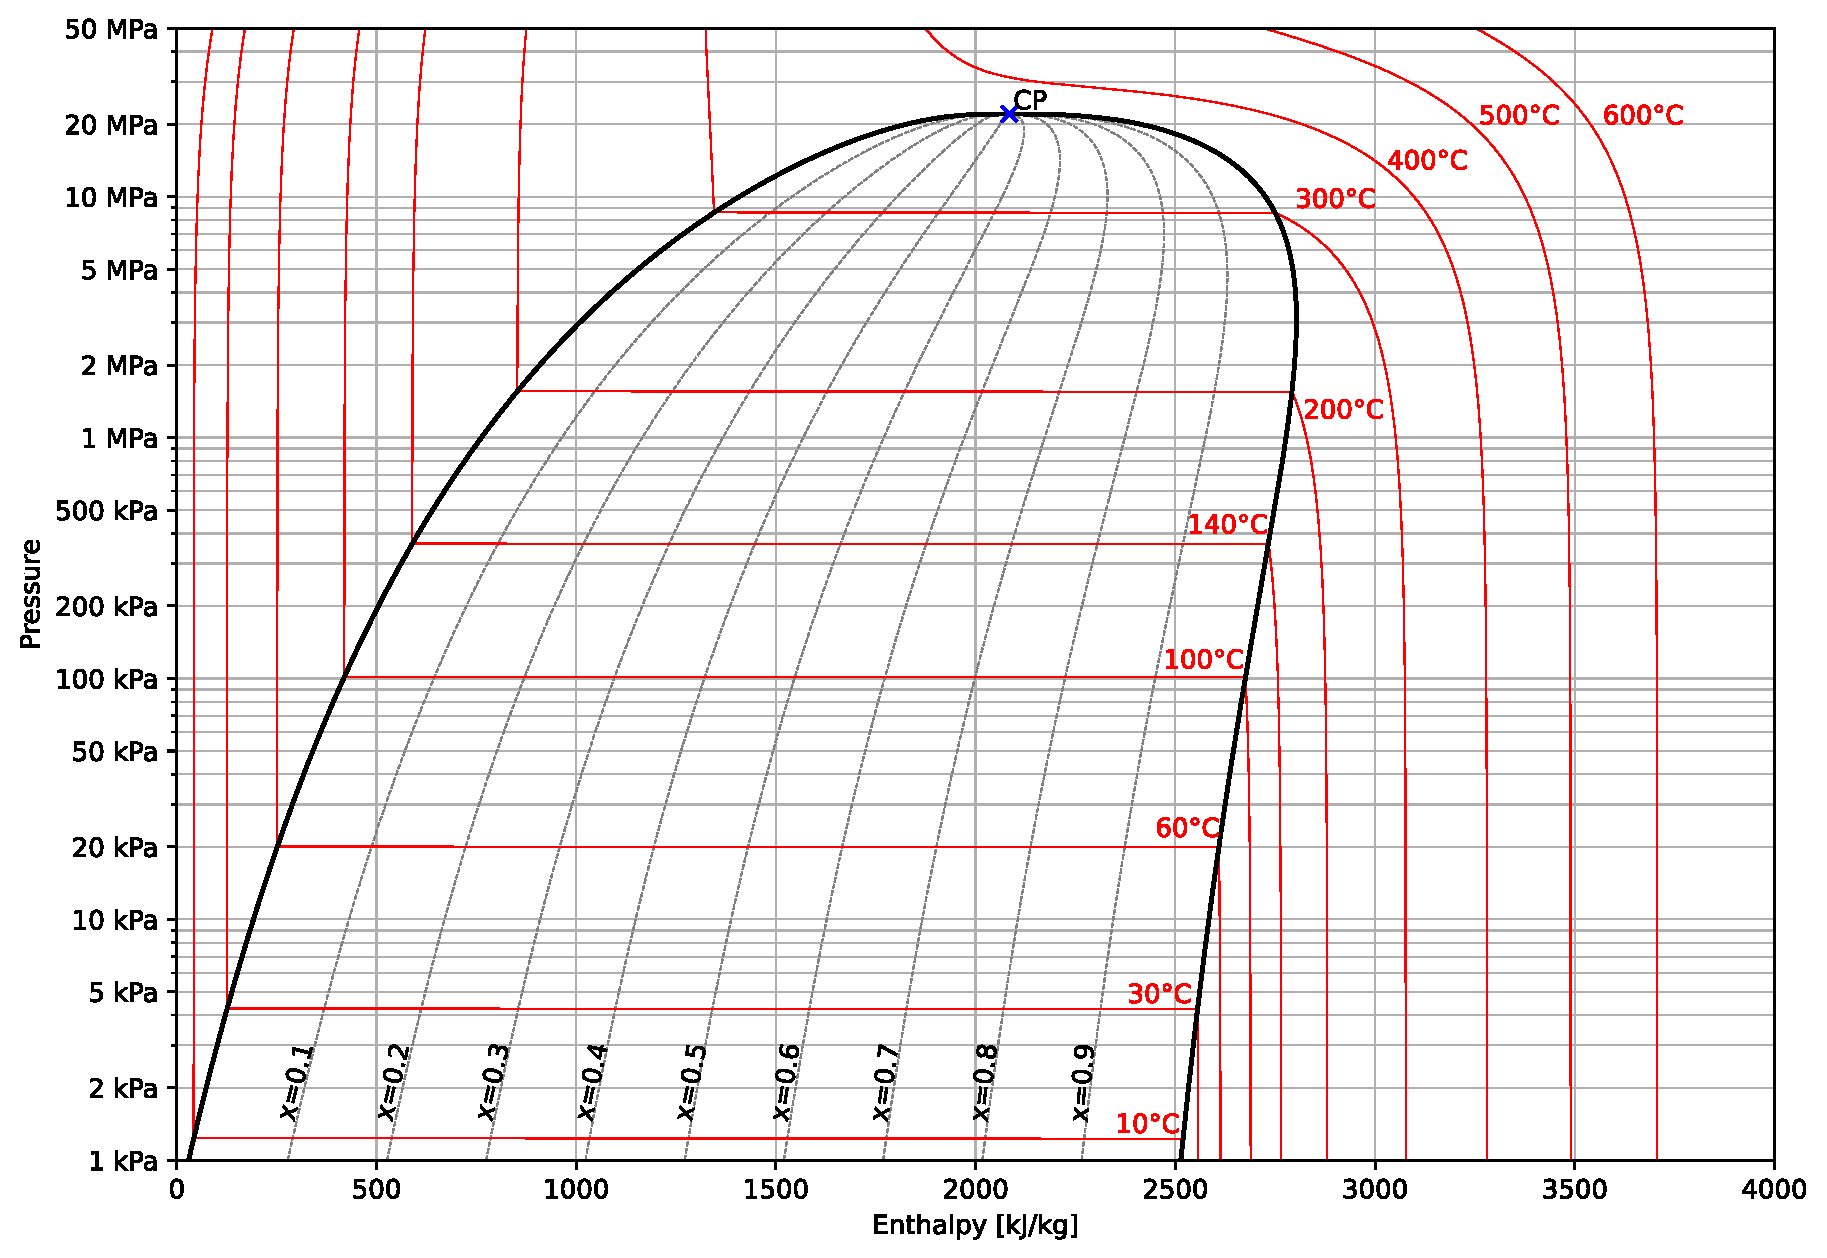
\includegraphics[width=.95\textheight, angle=90]{p-h_water}
\end{center}

% p-h diagram for Water
\section{Steam Enthalpy-Entropy ($h$-$s$) Diagram}
\begin{center}
  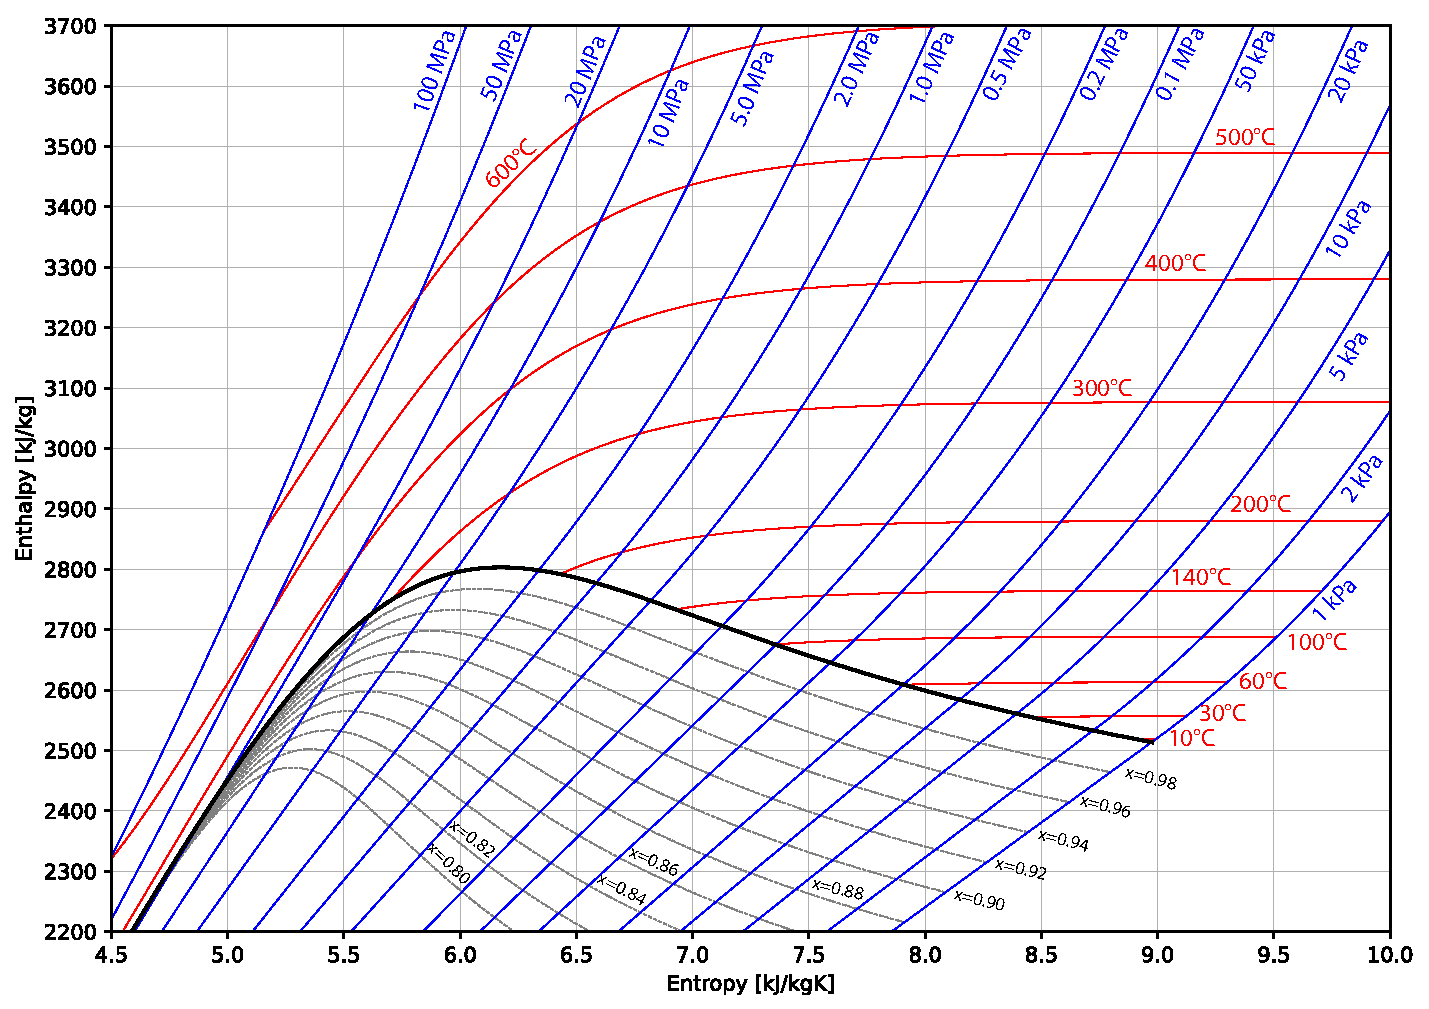
\includegraphics[width=.95\textheight, angle=90]{h-s_water}
\end{center}
\restoregeometry

\newgeometry{margin=1.0 in}
\chapter{R134a (Tetraflouroethane) Tables} \label{ch:appendixR134a}
Unless otherwise indicated, all data was sourced from the \href{https://webbook.nist.gov/chemistry/fluid/}{NIST Chemistry WebBook}, Accessed Dec. 2021.
\section{Saturation Properties for R134a - Temperature} \label{sec:R134aSatT}
\resetLTcolor
\begin{longtable}[!ht]{@{\zz\extracolsep{\fill}}cccccccccc}%{p{1cm}|p{1.5cm}|p{1.5cm}|p{1.5cm}|p{1.5cm}|p{1.5cm}|p{1.5cm}|p{1.5cm}|p{1.5cm}|p{1.5cm}}
%\begin{longtable}[!ht]{cccccccccc}%{p{1cm}|p{1.5cm}|p{1.5cm}|p{1.5cm}|p{1.5cm}|p{1.5cm}|p{1.5cm}|p{1.5cm}|p{1.5cm}|p{1.5cm}}
%    \centering
  %    \begin{tabular}{|l|l|l|l|l|l|l|l|l|l|}
  \multicolumn{1}{@{\fullwidthcolor{white}\extracolsep{\fill}}c}{\bf Temp.} & {\bf Pressure} & \multicolumn{2}{c}{\bf Density} & \multicolumn{2}{c}{\bf Int. Energy} & \multicolumn{2}{c}{\bf Enthalpy} & \multicolumn{2}{c}{\bf Entropy} \\
  \multicolumn{1}{@{\fullwidthcolor{white}\extracolsep{\fill}}c}{$T$} & $p$  & $\rho_f$  & $\rho_g$  & $u_f$  & $u_g$  & $h_f$ & $h_g$  & $s_f$  & $s_g$  \\ %
  \multicolumn{1}{@{\fullwidthcolor{white}\extracolsep{\fill}}c}{°C} & MPa & kg/$\rm m^3$ & kg/$\rm m^3$ & kJ/kg & kJ/kg & kJ/kg & kJ/kg & kJ/kgK & kJ/kgK  \\ \hline\endhead 
        -40 & 0.05121 & 1417.7 & 2.7695 & 148.11 & 355.51 & 148.14 & 374.00 & 0.7956 & 1.7643 \\ 
        -38 & 0.05682 & 1411.9 & 3.0529 & 150.62 & 356.66 & 150.66 & 375.27 & 0.8063 & 1.7615 \\ 
        -36 & 0.06291 & 1406.1 & 3.3590 & 153.14 & 357.81 & 153.18 & 376.54 & 0.8170 & 1.7588 \\ 
        -34 & 0.06951 & 1400.2 & 3.6890 & 155.66 & 358.96 & 155.71 & 377.80 & 0.8276 & 1.7563 \\ 
        -32 & 0.07666 & 1394.3 & 4.0441 & 158.19 & 360.11 & 158.25 & 379.06 & 0.8381 & 1.7538 \\ 
        -30 & 0.08438 & 1388.4 & 4.4259 & 160.73 & 361.25 & 160.79 & 380.32 & 0.8486 & 1.7515 \\ 
        -28 & 0.09270 & 1382.4 & 4.8356 & 163.28 & 362.40 & 163.34 & 381.57 & 0.8591 & 1.7492 \\ 
        -26 & 0.10167 & 1376.5 & 5.2748 & 165.83 & 363.55 & 165.90 & 382.82 & 0.8694 & 1.7471 \\ 
        -24 & 0.11130 & 1370.4 & 5.7450 & 168.39 & 364.70 & 168.47 & 384.07 & 0.8798 & 1.7451 \\ 
        -22 & 0.12165 & 1364.4 & 6.2477 & 170.96 & 365.84 & 171.05 & 385.32 & 0.8900 & 1.7432 \\ 
        -20 & 0.13273 & 1358.3 & 6.7845 & 173.54 & 366.99 & 173.64 & 386.55 & 0.9003 & 1.7413 \\ 
        -18 & 0.14460 & 1352.1 & 7.3571 & 176.12 & 368.13 & 176.23 & 387.79 & 0.9104 & 1.7396 \\ 
        -16 & 0.15728 & 1345.9 & 7.9673 & 178.72 & 369.28 & 178.83 & 389.02 & 0.9205 & 1.7379 \\ 
        -14 & 0.17082 & 1339.7 & 8.6168 & 181.32 & 370.41 & 181.44 & 390.24 & 0.9306 & 1.7363 \\ 
        -12 & 0.18524 & 1333.4 & 9.3074 & 183.93 & 371.55 & 184.07 & 391.46 & 0.9407 & 1.7348 \\ 
        -10 & 0.20060 & 1327.1 & 10.041 & 186.55 & 372.69 & 186.70 & 392.66 & 0.9507 & 1.7334 \\ 
        -8 & 0.21693 & 1320.8 & 10.820 & 189.17 & 373.82 & 189.34 & 393.87 & 0.9606 & 1.7320 \\ 
        -6 & 0.23428 & 1314.3 & 11.646 & 191.81 & 374.95 & 191.99 & 395.06 & 0.9705 & 1.7307 \\ 
        -4 & 0.25268 & 1307.9 & 12.521 & 194.45 & 376.07 & 194.65 & 396.25 & 0.9804 & 1.7294 \\ 
        -2 & 0.27217 & 1301.4 & 13.448 & 197.11 & 377.19 & 197.32 & 397.43 & 0.9902 & 1.7282 \\ 
        0 & 0.29280 & 1294.8 & 14.428 & 199.77 & 378.31 & 200.00 & 398.60 & 1.0000 & 1.7271 \\ 
        2 & 0.31462 & 1288.1 & 15.465 & 202.45 & 379.42 & 202.69 & 399.77 & 1.0098 & 1.7260 \\ 
        4 & 0.33766 & 1281.4 & 16.560 & 205.13 & 380.53 & 205.40 & 400.92 & 1.0195 & 1.7250 \\ 
        6 & 0.36198 & 1274.7 & 17.717 & 207.83 & 381.63 & 208.11 & 402.06 & 1.0292 & 1.7240 \\ 
        8 & 0.38761 & 1267.9 & 18.938 & 210.53 & 382.73 & 210.84 & 403.20 & 1.0388 & 1.7230 \\ 
        10 & 0.41461 & 1261.0 & 20.226 & 213.25 & 383.82 & 213.58 & 404.32 & 1.0485 & 1.7221 \\ 
        12 & 0.44301 & 1254.0 & 21.584 & 215.98 & 384.90 & 216.33 & 405.43 & 1.0581 & 1.7212 \\ 
        14 & 0.47288 & 1246.9 & 23.015 & 218.71 & 385.98 & 219.09 & 406.53 & 1.0677 & 1.7204 \\ 
        16 & 0.50425 & 1239.8 & 24.522 & 221.46 & 387.05 & 221.87 & 407.61 & 1.0772 & 1.7196 \\ 
        18 & 0.53718 & 1232.6 & 26.109 & 224.23 & 388.11 & 224.66 & 408.69 & 1.0867 & 1.7188 \\ 
        20 & 0.57171 & 1225.3 & 27.780 & 227.00 & 389.17 & 227.47 & 409.75 & 1.0962 & 1.7180 \\ 
        22 & 0.60789 & 1218.0 & 29.539 & 229.79 & 390.21 & 230.29 & 410.79 & 1.1057 & 1.7173 \\ 
        24 & 0.64578 & 1210.5 & 31.389 & 232.59 & 391.25 & 233.12 & 411.82 & 1.1152 & 1.7166 \\ 
        26 & 0.68543 & 1202.9 & 33.335 & 235.40 & 392.28 & 235.97 & 412.84 & 1.1246 & 1.7159 \\ 
        28 & 0.72688 & 1195.2 & 35.382 & 238.23 & 393.29 & 238.84 & 413.84 & 1.1341 & 1.7152 \\ 
        30 & 0.77020 & 1187.5 & 37.535 & 241.07 & 394.30 & 241.72 & 414.82 & 1.1435 & 1.7145 \\ 
        32 & 0.81543 & 1179.6 & 39.799 & 243.93 & 395.29 & 244.62 & 415.78 & 1.1529 & 1.7138 \\ 
        34 & 0.86263 & 1171.6 & 42.180 & 246.80 & 396.27 & 247.54 & 416.72 & 1.1623 & 1.7131 \\ 
        36 & 0.91185 & 1163.4 & 44.683 & 249.69 & 397.24 & 250.48 & 417.65 & 1.1717 & 1.7124 \\ 
        38 & 0.96315 & 1155.1 & 47.316 & 252.60 & 398.19 & 253.43 & 418.55 & 1.1811 & 1.7118 \\ 
        40 & 1.0166 & 1146.7 & 50.085 & 255.52 & 399.13 & 256.41 & 419.43 & 1.1905 & 1.7111 \\ 
        42 & 1.0722 & 1138.2 & 52.998 & 258.46 & 400.05 & 259.41 & 420.28 & 1.1999 & 1.7103 \\ 
        44 & 1.1301 & 1129.5 & 56.064 & 261.42 & 400.96 & 262.43 & 421.11 & 1.2092 & 1.7096 \\ 
        46 & 1.1903 & 1120.6 & 59.292 & 264.40 & 401.84 & 265.47 & 421.92 & 1.2186 & 1.7089 \\ 
        48 & 1.2529 & 1111.5 & 62.690 & 267.41 & 402.71 & 268.53 & 422.69 & 1.2280 & 1.7081 \\ 
        50 & 1.3179 & 1102.3 & 66.272 & 270.43 & 403.55 & 271.62 & 423.44 & 1.2375 & 1.7072 \\ 
        52 & 1.3854 & 1092.9 & 70.047 & 273.47 & 404.37 & 274.74 & 424.15 & 1.2469 & 1.7064 \\ 
        54 & 1.4555 & 1083.2 & 74.030 & 276.54 & 405.17 & 277.89 & 424.83 & 1.2563 & 1.7055 \\ 
        56 & 1.5282 & 1073.4 & 78.235 & 279.64 & 405.94 & 281.06 & 425.47 & 1.2658 & 1.7045 \\ 
        58 & 1.6036 & 1063.2 & 82.679 & 282.76 & 406.67 & 284.27 & 426.07 & 1.2753 & 1.7035 \\ 
        60 & 1.6818 & 1052.9 & 87.379 & 285.91 & 407.38 & 287.50 & 426.63 & 1.2848 & 1.7024 \\ 
        62 & 1.7628 & 1042.2 & 92.358 & 289.09 & 408.06 & 290.78 & 427.14 & 1.2944 & 1.7013 \\ 
        64 & 1.8467 & 1031.2 & 97.637 & 292.30 & 408.69 & 294.09 & 427.61 & 1.3040 & 1.7000 \\ 
        66 & 1.9337 & 1020.0 & 103.24 & 295.55 & 409.29 & 297.44 & 428.02 & 1.3137 & 1.6987 \\ 
        68 & 2.0237 & 1008.3 & 109.21 & 298.83 & 409.84 & 300.84 & 428.36 & 1.3234 & 1.6972 \\ 
        70 & 2.1168 & 996.25 & 115.57 & 302.16 & 410.33 & 304.28 & 428.65 & 1.3332 & 1.6956 \\ 
        72 & 2.2132 & 983.76 & 122.37 & 305.53 & 410.78 & 307.78 & 428.86 & 1.3430 & 1.6939 \\ 
        74 & 2.3130 & 970.78 & 129.65 & 308.95 & 411.16 & 311.33 & 429.00 & 1.3530 & 1.6920 \\ 
        76 & 2.4161 & 957.25 & 137.48 & 312.42 & 411.47 & 314.94 & 429.04 & 1.3631 & 1.6899 \\ 
        78 & 2.5228 & 943.10 & 145.93 & 315.95 & 411.70 & 318.63 & 428.98 & 1.3733 & 1.6876 \\ 
        80 & 2.6332 & 928.24 & 155.08 & 319.55 & 411.83 & 322.39 & 428.81 & 1.3836 & 1.6850 \\ 
        82 & 2.7473 & 912.56 & 165.05 & 323.23 & 411.87 & 326.24 & 428.51 & 1.3942 & 1.6821 \\ 
        84 & 2.8653 & 895.91 & 175.97 & 327.00 & 411.77 & 330.20 & 428.05 & 1.4049 & 1.6789 \\ 
        86 & 2.9874 & 878.10 & 188.05 & 330.88 & 411.53 & 334.28 & 427.42 & 1.4159 & 1.6752 \\ 
        88 & 3.1136 & 858.86 & 201.52 & 334.89 & 411.10 & 338.51 & 426.55 & 1.4273 & 1.6710 \\ 
        90 & 3.2442 & 837.83 & 216.76 & 339.06 & 410.45 & 342.93 & 425.42 & 1.4390 & 1.6662 \\ 
        92 & 3.3793 & 814.43 & 234.31 & 343.44 & 409.49 & 347.59 & 423.92 & 1.4514 & 1.6604 \\ 
        94 & 3.5193 & 787.75 & 255.08 & 348.11 & 408.13 & 352.58 & 421.92 & 1.4645 & 1.6534 \\ 
        96 & 3.6645 & 756.09 & 280.73 & 353.23 & 406.13 & 358.07 & 419.18 & 1.4789 & 1.6445 \\ 
        98 & 3.8152 & 715.51 & 315.13 & 359.14 & 403.03 & 364.47 & 415.14 & 1.4957 & 1.6322 \\ 
        100 & 3.9724 & 651.18 & 373.01 & 367.20 & 397.03 & 373.30 & 407.68 & 1.5188 & 1.6109 \\ 
        101.06 & 4.0591 & 511.90 & 511.90 & 381.71 & 381.71 & 389.64 & 389.64 & 1.5621 & 1.5621 

%    \end{tabular}
\end{longtable}
\newpage
\section{Saturation Properties for R134a - Pressure} \label{sec:R134aSatP}
\resetLTcolor

\begin{longtable}[!ht]{@{\zz\extracolsep{\fill}}cccccccccc}%{p{1cm}|p{1.5cm}|p{1.5cm}|p{1.5cm}|p{1.5cm}|p{1.5cm}|p{1.5cm}|p{1.5cm}|p{1.5cm}|p{1.5cm}}
%\begin{longtable}[!ht]{cccccccccc}%{p{1cm}|p{1.5cm}|p{1.5cm}|p{1.5cm}|p{1.5cm}|p{1.5cm}|p{1.5cm}|p{1.5cm}|p{1.5cm}|p{1.5cm}}
%    \centering
  %    \begin{tabular}{|l|l|l|l|l|l|l|l|l|l|}
  \multicolumn{1}{@{\fullwidthcolor{white}\extracolsep{\fill}}c}{\bf Pressure} & {\bf Temp.} & \multicolumn{2}{c}{\bf Density} & \multicolumn{2}{c}{\bf Int. Energy} & \multicolumn{2}{c}{\bf Enthalpy} & \multicolumn{2}{c}{\bf Entropy} \\
  \multicolumn{1}{@{\fullwidthcolor{white}\extracolsep{\fill}}c}{$p$} & $T$  & $\rho_f$  & $\rho_g$  & $u_f$  & $u_g$  & $h_f$ & $h_g$  & $s_f$  & $s_g$  \\ %
  \multicolumn{1}{@{\fullwidthcolor{white}\extracolsep{\fill}}c}{MPa} & °C & kg/$\rm m^3$ & kg/$\rm m^3$ & kJ/kg & kJ/kg & kJ/kg & kJ/kg & kJ/kgK & kJ/kgK  \\ \hline\endhead 
        0.02 & -56.41 & 1464.3 & 1.1484 & 127.75 & 346.17 & 127.77 & 363.58 & 0.7051 & 1.7931 \\ 
        0.04 & -44.60 & 1430.9 & 2.1973 & 142.36 & 352.88 & 142.39 & 371.09 & 0.7707 & 1.7713 \\ 
        0.06 & -36.94 & 1408.8 & 3.2131 & 151.96 & 357.27 & 152.00 & 375.94 & 0.8120 & 1.7601 \\ 
        0.08 & -31.12 & 1391.7 & 4.2096 & 159.31 & 360.61 & 159.37 & 379.62 & 0.8428 & 1.7528 \\ 
        0.10 & -26.36 & 1377.5 & 5.1932 & 165.37 & 363.34 & 165.44 & 382.60 & 0.8676 & 1.7475 \\ 
        0.12 & -22.31 & 1365.3 & 6.1677 & 170.56 & 365.67 & 170.65 & 385.12 & 0.8884 & 1.7435 \\ 
        0.14 & -18.76 & 1354.5 & 7.1353 & 175.14 & 367.70 & 175.24 & 387.32 & 0.9066 & 1.7402 \\ 
        0.16 & -15.59 & 1344.7 & 8.0979 & 179.25 & 369.51 & 179.37 & 389.27 & 0.9226 & 1.7376 \\ 
        0.18 & -12.71 & 1335.7 & 9.0566 & 183.00 & 371.15 & 183.13 & 391.02 & 0.9371 & 1.7353 \\ 
        0.20 & -10.08 & 1327.4 & 10.012 & 186.45 & 372.64 & 186.60 & 392.62 & 0.9503 & 1.7334 \\ 
        0.22 & -7.64 & 1319.6 & 10.966 & 189.65 & 374.02 & 189.82 & 394.09 & 0.9624 & 1.7317 \\ 
        0.24 & -5.37 & 1312.3 & 11.918 & 192.65 & 375.30 & 192.83 & 395.44 & 0.9736 & 1.7303 \\ 
        0.26 & -3.24 & 1305.4 & 12.869 & 195.47 & 376.50 & 195.67 & 396.70 & 0.9841 & 1.7290 \\ 
        0.28 & -1.23 & 1298.8 & 13.820 & 198.14 & 377.62 & 198.35 & 397.89 & 0.9940 & 1.7278 \\ 
        0.30 & 0.67 & 1292.6 & 14.770 & 200.67 & 378.68 & 200.90 & 399.00 & 1.0033 & 1.7267 \\ 
        0.32 & 2.48 & 1286.5 & 15.721 & 203.09 & 379.69 & 203.34 & 400.04 & 1.0121 & 1.7257 \\ 
        0.34 & 4.20 & 1280.8 & 16.671 & 205.40 & 380.64 & 205.66 & 401.03 & 1.0204 & 1.7249 \\ 
        0.36 & 5.84 & 1275.2 & 17.623 & 207.61 & 381.54 & 207.90 & 401.97 & 1.0284 & 1.7240 \\ 
        0.38 & 7.42 & 1269.9 & 18.575 & 209.74 & 382.41 & 210.04 & 402.87 & 1.0360 & 1.7233 \\ 
        0.40 & 8.93 & 1264.7 & 19.529 & 211.79 & 383.24 & 212.11 & 403.72 & 1.0433 & 1.7226 \\ 
        0.45 & 12.48 & 1252.3 & 21.918 & 216.63 & 385.16 & 216.99 & 405.69 & 1.0604 & 1.7210 \\ 
        0.50 & 15.74 & 1240.8 & 24.317 & 221.10 & 386.91 & 221.50 & 407.47 & 1.0759 & 1.7197 \\ 
        0.55 & 18.75 & 1229.9 & 26.729 & 225.27 & 388.51 & 225.72 & 409.09 & 1.0903 & 1.7185 \\ 
        0.60 & 21.57 & 1219.5 & 29.155 & 229.19 & 389.99 & 229.68 & 410.57 & 1.1037 & 1.7175 \\ 
        0.65 & 24.22 & 1209.7 & 31.596 & 232.89 & 391.36 & 233.43 & 411.94 & 1.1162 & 1.7165 \\ 
        0.70 & 26.71 & 1200.2 & 34.054 & 236.41 & 392.64 & 236.99 & 413.20 & 1.1280 & 1.7156 \\ 
%        0.75 & 29.08 & 1191.1 & 36.530 & 239.76 & 393.84 & 240.39 & 414.37 & 1.1392 & 1.7148 \\ 
        0.80 & 31.33 & 1182.2 & 39.025 & 242.97 & 394.96 & 243.65 & 415.46 & 1.1497 & 1.7140 \\ 
%        0.85 & 33.47 & 1173.7 & 41.541 & 246.05 & 396.02 & 246.77 & 416.48 & 1.1598 & 1.7133 \\ 
        0.90 & 35.53 & 1165.4 & 44.078 & 249.01 & 397.01 & 249.78 & 417.43 & 1.1695 & 1.7126 \\ 
%        0.95 & 37.50 & 1157.2 & 46.638 & 251.86 & 397.95 & 252.69 & 418.32 & 1.1787 & 1.7119 \\ 
        1.0 & 39.39 & 1149.3 & 49.222 & 254.63 & 398.85 & 255.50 & 419.16 & 1.1876 & 1.7113 \\ 
        1.1 & 42.97 & 1134.0 & 54.465 & 259.90 & 400.49 & 260.87 & 420.69 & 1.2044 & 1.7100 \\ 
        1.2 & 46.32 & 1119.2 & 59.815 & 264.88 & 401.98 & 265.95 & 422.04 & 1.2201 & 1.7087 \\ 
        1.3 & 49.46 & 1104.8 & 65.280 & 269.60 & 403.32 & 270.78 & 423.24 & 1.2349 & 1.7075 \\ 
        1.4 & 52.42 & 1090.9 & 70.870 & 274.12 & 404.54 & 275.40 & 424.30 & 1.2489 & 1.7062 \\ 
        1.5 & 55.23 & 1077.2 & 76.595 & 278.45 & 405.64 & 279.84 & 425.23 & 1.2622 & 1.7049 \\ 
        1.6 & 57.91 & 1063.7 & 82.464 & 282.61 & 406.64 & 284.11 & 426.04 & 1.2748 & 1.7036 \\ 
%        1.7 & 60.46 & 1050.5 & 88.489 & 286.63 & 407.54 & 288.25 & 426.75 & 1.2870 & 1.7022 \\ 
        1.8 & 62.90 & 1037.3 & 94.682 & 290.52 & 408.35 & 292.26 & 427.36 & 1.2987 & 1.7007 \\ 
%        1.9 & 65.23 & 1024.3 & 101.06 & 294.30 & 409.06 & 296.15 & 427.87 & 1.3100 & 1.6992 \\ 
        2.0 & 67.48 & 1011.4 & 107.63 & 297.98 & 409.70 & 299.95 & 428.28 & 1.3209 & 1.6976 \\ 
        2.2 & 71.73 & 985.47 & 121.42 & 305.07 & 410.72 & 307.30 & 428.84 & 1.3417 & 1.6941 \\ 
        2.4 & 75.69 & 959.38 & 136.24 & 311.88 & 411.42 & 314.38 & 429.04 & 1.3615 & 1.6902 \\ 
        2.6 & 79.41 & 932.74 & 152.28 & 318.47 & 411.80 & 321.26 & 428.88 & 1.3805 & 1.6858 \\ 
        2.8 & 82.90 & 905.19 & 169.84 & 324.92 & 411.84 & 328.01 & 428.33 & 1.3990 & 1.6807 \\ 
        3.0 & 86.20 & 876.21 & 189.35 & 331.28 & 411.49 & 334.70 & 427.34 & 1.4171 & 1.6748 \\ 
        3.2 & 89.33 & 845.09 & 211.44 & 337.64 & 410.70 & 341.43 & 425.83 & 1.4350 & 1.6679 \\ 
        3.4 & 92.30 & 810.67 & 237.19 & 344.12 & 409.32 & 348.31 & 423.65 & 1.4533 & 1.6595 \\ 
        3.6 & 95.12 & 770.79 & 268.69 & 350.91 & 407.11 & 355.58 & 420.50 & 1.4724 & 1.6487 \\ 
        3.8 & 97.80 & 720.15 & 311.11 & 358.50 & 403.41 & 363.77 & 415.63 & 1.4939 & 1.6336 \\ 
        4.0 & 100.34 & 632.87 & 390.23 & 369.25 & 395.13 & 375.57 & 405.38 & 1.5247 & 1.6046 \\ 
        4.0591 & 101.06 & 511.90 & 511.90 & 381.71 & 381.71 & 389.64 & 389.64 & 1.5621 & 1.5621

%    \end{tabular}
\end{longtable}


\section{Superheated Vapor Properties for Refrigerant R134a}
\resetLTcolor

% 60 kPa and 100 kPa
\begin{longtable}[!ht]{@{\zz\extracolsep{\fill}}c|cccc|cccc}
  \multicolumn{1}{@{\fullwidthcolor{white}\extracolsep{\fill}}c}{} & \multicolumn{4}{c|}{$p$ = 0.06 MPa ($T_{sat}$ = -36.9°C)} & \multicolumn{4}{c}{$p$ = 0.10 MPa ($T_{sat}$ = -26.4°C)} \\ \hline
  \multicolumn{1}{@{\fullwidthcolor{white}\extracolsep{\fill}}c|}{\bf Temp.} & {\bf Density} & {\bf Energy} & {\bf Enthalpy} & {\bf Entropy}
  & {\bf Density} & {\bf Energy} & {\bf Enthalpy} & {\bf Entropy} \\
  \multicolumn{1}{@{\fullwidthcolor{white}\extracolsep{\fill}}c|}{$T$} & $\rho$ & $u$ & $h$ & $s$ & $\rho$ & $u$ & $h$ & $s$ \\ %
  \multicolumn{1}{@{\fullwidthcolor{white}\extracolsep{\fill}}c|}{°C} & kg/$\rm m^3$ & kJ/kg & kJ/kg & kJ/kgK & kg/$\rm m^3$ & kJ/kg & kJ/kg & kJ/kgK \\ \hline\endhead 
         Sat. & 3.2131 & 357.27 & 375.94 & 1.7601 & 5.1933 & 363.34 & 382.60 & 1.7475 \\
        -30 & 3.1105 & 361.93 & 381.22 & 1.7821 & ~ & ~ & ~ & ~ \\ 
        -20 & 2.9755 & 368.74 & 388.91 & 1.8131 & 5.0401 & 367.81 & 387.65 & 1.7677 \\
        -10 & 2.8532 & 375.70 & 396.73 & 1.8433 & 4.8208 & 374.89 & 395.64 & 1.7986 \\
        0 & 2.7415 & 382.80 & 404.69 & 1.8730 & 4.6232 & 382.10 & 403.73 & 1.8288 \\ 
        10 & 2.6390 & 390.07 & 412.81 & 1.9022 & 4.4433 & 389.45 & 411.95 & 1.8584 \\ 
        20 & 2.5444 & 397.50 & 421.08 & 1.9310 & 4.2784 & 396.94 & 420.31 & 1.8874 \\ 
        30 & 2.4567 & 405.10 & 429.52 & 1.9593 & 4.1266 & 404.59 & 428.82 & 1.9159 \\ 
        40 & 2.3752 & 412.86 & 438.12 & 1.9872 & 3.9860 & 412.40 & 437.49 & 1.9441 \\ 
        50 & 2.2991 & 420.79 & 446.88 & 2.0147 & 3.8554 & 420.37 & 446.30 & 1.9718 \\ 
        60 & 2.2280 & 428.88 & 455.81 & 2.0419 & 3.7336 & 428.49 & 455.28 & 1.9991 \\ 
        70 & 2.1613 & 437.14 & 464.90 & 2.0688 & 3.6198 & 436.78 & 464.41 & 2.0261 \\ 
        80 & 2.0986 & 445.56 & 474.15 & 2.0954 & 3.5130 & 445.23 & 473.70 & 2.0528 \\ 
        90 & 2.0395 & 454.14 & 483.56 & 2.1216 & 3.4126 & 453.84 & 483.14 & 2.0792 \\ 
        100 & 1.9837 & 462.89 & 493.14 & 2.1477 & 3.3181 & 462.61 & 492.74 & 2.1053

\end{longtable}

% 140 kPa and 180 kPa
\begin{longtable}[!ht]{@{\zz\extracolsep{\fill}}c|cccc|cccc}
  \multicolumn{1}{@{\fullwidthcolor{white}\extracolsep{\fill}}c}{} & \multicolumn{4}{c|}{$p$ = 0.14 MPa ($T_{sat}$ = -18.8°C)} & \multicolumn{4}{c}{$p$ = 0.18 MPa ($T_{sat}$ = -12.7°C)} \\ \hline
  \multicolumn{1}{@{\fullwidthcolor{white}\extracolsep{\fill}}c|}{\bf Temp.} & {\bf Density} & {\bf Energy} & {\bf Enthalpy} & {\bf Entropy}
  & {\bf Density} & {\bf Energy} & {\bf Enthalpy} & {\bf Entropy} \\
  \multicolumn{1}{@{\fullwidthcolor{white}\extracolsep{\fill}}c|}{$T$} & $\rho$ & $u$ & $h$ & $s$ & $\rho$ & $u$ & $h$ & $s$ \\ %
  \multicolumn{1}{@{\fullwidthcolor{white}\extracolsep{\fill}}c|}{°C} & kg/$\rm m^3$ & kJ/kg & kJ/kg & kJ/kgK & kg/$\rm m^3$ & kJ/kg & kJ/kg & kJ/kgK \\ \hline\endhead 
         Sat. & 7.1353 & 367.70 & 387.32 & 1.7402 & 9.0566 & 371.15 & 391.02 & 1.7353 \\
        -10 & 6.8467 & 374.05 & 394.50 & 1.7680 & 8.9369 & 373.17 & 393.31 & 1.7441 \\
        0 & 6.5517 & 381.37 & 402.74 & 1.7987 & 8.5310 & 380.62 & 401.72 & 1.7754 \\  
        10 & 6.2861 & 388.81 & 411.08 & 1.8287 & 8.1699 & 388.15 & 410.18 & 1.8059 \\ 
        20 & 6.0446 & 396.37 & 419.53 & 1.8580 & 7.8445 & 395.79 & 418.73 & 1.8355 \\ 
        30 & 5.8234 & 404.08 & 428.12 & 1.8868 & 7.5484 & 403.55 & 427.40 & 1.8646 \\ 
        40 & 5.6197 & 411.93 & 436.84 & 1.9151 & 7.2772 & 411.46 & 436.19 & 1.8931 \\ 
        50 & 5.4312 & 419.94 & 445.72 & 1.9430 & 7.0273 & 419.51 & 445.12 & 1.9212 \\ 
        60 & 5.2561 & 428.10 & 454.74 & 1.9705 & 6.7959 & 427.71 & 454.20 & 1.9489 \\ 
        70 & 5.0928 & 436.42 & 463.91 & 1.9977 & 6.5808 & 436.06 & 463.41 & 1.9761 \\ 
        80 & 4.9401 & 444.90 & 473.24 & 2.0244 & 6.3802 & 444.56 & 472.78 & 2.0030 \\ 
        90 & 4.7968 & 453.53 & 482.72 & 2.0509 & 6.1923 & 453.22 & 482.29 & 2.0296 \\ 
        100 & 4.6621 & 462.32 & 492.35 & 2.0771 & 6.0160 & 462.03 & 491.95 & 2.0558 

\end{longtable}

% 200 kPa and 240 kPa
\begin{longtable}[!ht]{@{\zz\extracolsep{\fill}}c|cccc|cccc}
  \multicolumn{1}{@{\fullwidthcolor{white}\extracolsep{\fill}}c}{} & \multicolumn{4}{c|}{$p$ = 0.20 MPa ($T_{sat}$ = -10.1°C)} & \multicolumn{4}{c}{$p$ = 0.24 MPa ($T_{sat}$ = -5.4°C)} \\ \hline
  \multicolumn{1}{@{\fullwidthcolor{white}\extracolsep{\fill}}c|}{\bf Temp.} & {\bf Density} & {\bf Energy} & {\bf Enthalpy} & {\bf Entropy}
  & {\bf Density} & {\bf Energy} & {\bf Enthalpy} & {\bf Entropy} \\
  \multicolumn{1}{@{\fullwidthcolor{white}\extracolsep{\fill}}c|}{$T$} & $\rho$ & $u$ & $h$ & $s$ & $\rho$ & $u$ & $h$ & $s$ \\ %
  \multicolumn{1}{@{\fullwidthcolor{white}\extracolsep{\fill}}c|}{°C} & kg/$\rm m^3$ & kJ/kg & kJ/kg & kJ/kgK & kg/$\rm m^3$ & kJ/kg & kJ/kg & kJ/kgK \\ \hline\endhead 
         Sat. & 10.012 & 372.64 & 392.62 & 1.7334 & 11.918 & 375.30 & 395.44 & 1.7303 \\
        -10 & 10.009 & 372.70 & 392.68 & 1.7337 & ~ & ~ & ~ & ~ \\
        0 & 9.5410 & 380.23 & 401.20 & 1.7654 & 11.605 & 379.43 & 400.11 & 1.7475 \\  
        10 & 9.1281 & 387.81 & 409.73 & 1.7961 & 11.079 & 387.13 & 408.79 & 1.7787 \\ 
        20 & 8.7577 & 395.49 & 418.33 & 1.8259 & 10.612 & 394.89 & 417.51 & 1.8090 \\ 
        30 & 8.4220 & 403.29 & 427.04 & 1.8551 & 10.192 & 402.75 & 426.30 & 1.8385 \\ 
        40 & 8.1152 & 411.22 & 435.87 & 1.8838 & 9.8102 & 410.74 & 435.20 & 1.8674 \\ 
        50 & 7.8332 & 419.29 & 444.83 & 1.9120 & 9.4609 & 418.86 & 444.22 & 1.8957 \\ 
        60 & 7.5725 & 427.51 & 453.92 & 1.9397 & 9.1393 & 427.11 & 453.37 & 1.9236 \\ 
        70 & 7.3306 & 435.88 & 463.16 & 1.9670 & 8.8417 & 435.51 & 462.65 & 1.9511 \\ 
        80 & 7.1051 & 444.39 & 472.54 & 1.9939 & 8.5652 & 444.06 & 472.08 & 1.9781 \\ 
        90 & 6.8944 & 453.06 & 482.07 & 2.0206 & 8.3072 & 452.75 & 481.64 & 2.0048 \\ 
        100 & 6.6967 & 461.88 & 491.75 & 2.0468 & 8.0658 & 461.59 & 491.35 & 2.0312

\end{longtable}

% 280 kPa and 320 kPa
\begin{longtable}[!ht]{@{\zz\extracolsep{\fill}}c|cccc|cccc}
  \multicolumn{1}{@{\fullwidthcolor{white}\extracolsep{\fill}}c}{} & \multicolumn{4}{c|}{$p$ = 0.28 MPa ($T_{sat}$ = -1.2°C)} & \multicolumn{4}{c}{$p$ = 0.32 MPa ($T_{sat}$ = 2.5°C)} \\ \hline
  \multicolumn{1}{@{\fullwidthcolor{white}\extracolsep{\fill}}c|}{\bf Temp.} & {\bf Density} & {\bf Energy} & {\bf Enthalpy} & {\bf Entropy}
  & {\bf Density} & {\bf Energy} & {\bf Enthalpy} & {\bf Entropy} \\
  \multicolumn{1}{@{\fullwidthcolor{white}\extracolsep{\fill}}c|}{$T$} & $\rho$ & $u$ & $h$ & $s$ & $\rho$ & $u$ & $h$ & $s$ \\ %
  \multicolumn{1}{@{\fullwidthcolor{white}\extracolsep{\fill}}c|}{°C} & kg/$\rm m^3$ & kJ/kg & kJ/kg & kJ/kgK & kg/$\rm m^3$ & kJ/kg & kJ/kg & kJ/kgK \\ \hline\endhead 
         Sat. & 13.820 & 377.62 & 397.89 & 1.7278 & 15.721 & 379.69 & 400.04 & 1.7257 \\
        0 & 13.733 & 378.59 & 398.98 & 1.7318 & ~ & ~ & ~ & ~ \\ 
        10 & 13.079 & 386.42 & 407.83 & 1.7636 & 15.131 & 385.68 & 406.83 & 1.7501 \\ 
        20 & 12.505 & 394.27 & 416.66 & 1.7943 & 14.440 & 393.64 & 415.80 & 1.7812 \\ 
        30 & 11.994 & 402.21 & 425.55 & 1.8241 & 13.829 & 401.65 & 424.79 & 1.8113 \\ 
        40 & 11.532 & 410.25 & 434.53 & 1.8532 & 13.280 & 409.75 & 433.85 & 1.8407 \\ 
        50 & 11.111 & 418.41 & 443.61 & 1.8818 & 12.783 & 417.96 & 443.00 & 1.8695 \\ 
        60 & 10.725 & 426.71 & 452.81 & 1.9098 & 12.330 & 426.30 & 452.25 & 1.8977 \\ 
        70 & 10.369 & 435.14 & 462.14 & 1.9374 & 11.912 & 434.77 & 461.63 & 1.9254 \\ 
        80 & 10.039 & 443.71 & 471.61 & 1.9646 & 11.527 & 443.37 & 471.13 & 1.9527 \\ 
        90 & 9.7319 & 452.43 & 481.20 & 1.9914 & 11.169 & 452.11 & 480.77 & 1.9796 \\ 
        100 & 9.4452 & 461.30 & 490.94 & 2.0178 & 10.835 & 461.00 & 490.54 & 2.0062 \\
        110 & 9.1765 & 470.31 & 500.82 & 2.0440 & 10.523 & 470.03 & 500.44 & 2.0324 \\
        120 & 8.9241 & 479.47 & 510.85 & 2.0698 & 10.230 & 479.21 & 510.49 & 2.0583

\end{longtable}

% 400 kPa and 500 kPa
\begin{longtable}[!ht]{@{\zz\extracolsep{\fill}}c|cccc|cccc}
  \multicolumn{1}{@{\fullwidthcolor{white}\extracolsep{\fill}}c}{} & \multicolumn{4}{c|}{$p$ = 0.40 MPa ($T_{sat}$ = 8.9°C)} & \multicolumn{4}{c}{$p$ = 0.50 MPa ($T_{sat}$ = 15.7°C)} \\ \hline
  \multicolumn{1}{@{\fullwidthcolor{white}\extracolsep{\fill}}c|}{\bf Temp.} & {\bf Density} & {\bf Energy} & {\bf Enthalpy} & {\bf Entropy}
  & {\bf Density} & {\bf Energy} & {\bf Enthalpy} & {\bf Entropy} \\
  \multicolumn{1}{@{\fullwidthcolor{white}\extracolsep{\fill}}c|}{$T$} & $\rho$ & $u$ & $h$ & $s$ & $\rho$ & $u$ & $h$ & $s$ \\ %
  \multicolumn{1}{@{\fullwidthcolor{white}\extracolsep{\fill}}c|}{°C} & kg/$\rm m^3$ & kJ/kg & kJ/kg & kJ/kgK & kg/$\rm m^3$ & kJ/kg & kJ/kg & kJ/kgK \\ \hline\endhead 
         Sat. & 19.529 & 383.24 & 403.72 & 1.7226 & 24.317 & 386.91 & 407.47 & 1.7197 \\
        10 & 19.415 & 384.12 & 404.72 & 1.7261 & ~ & ~ & ~ & ~ \\ 
        20 & 18.446 & 392.32 & 414.01 & 1.7584 & 23.744 & 390.55 & 411.61 & 1.7339 \\ 
        30 & 17.607 & 400.50 & 423.22 & 1.7893 & 22.554 & 398.99 & 421.16 & 1.7659 \\ 
        40 & 16.865 & 408.73 & 432.45 & 1.8192 & 21.526 & 407.40 & 430.63 & 1.7967 \\ 
        50 & 16.201 & 417.05 & 441.74 & 1.8484 & 20.619 & 415.86 & 440.11 & 1.8265 \\ 
        60 & 15.600 & 425.47 & 451.11 & 1.8770 & 19.808 & 424.40 & 449.64 & 1.8555 \\ 
        70 & 15.050 & 434.01 & 460.58 & 1.9050 & 19.074 & 433.04 & 459.25 & 1.8839 \\ 
        80 & 14.546 & 442.67 & 470.17 & 1.9325 & 18.406 & 441.78 & 468.95 & 1.9118 \\ 
        90 & 14.080 & 451.47 & 479.88 & 1.9596 & 17.792 & 450.65 & 478.75 & 1.9392 \\ 
        100 & 13.647 & 460.41 & 489.72 & 1.9864 & 17.225 & 459.65 & 488.67 & 1.9661 \\
        110 & 13.244 & 469.48 & 499.68 & 2.0127 & 16.700 & 468.78 & 498.72 & 1.9927 \\
        120 & 12.867 & 478.69 & 509.78 & 2.0387 & 16.211 & 478.04 & 508.88 & 2.0189 \\
        130 & 12.513 & 488.05 & 520.02 & 2.0645 & 15.753 & 487.44 & 519.18 & 2.0447 \\
        140 & 12.181 & 497.55 & 530.39 & 2.0899 & 15.324 & 496.98 & 529.60 & 2.0703 

\end{longtable}

% 600 kPa and 700 kPa
\begin{longtable}[!ht]{@{\zz\extracolsep{\fill}}c|cccc|cccc}
  \multicolumn{1}{@{\fullwidthcolor{white}\extracolsep{\fill}}c}{} & \multicolumn{4}{c|}{$p$ = 0.60 MPa ($T_{sat}$ = 21.6°C)} & \multicolumn{4}{c}{$p$ = 0.70 MPa ($T_{sat}$ = 26.7°C)} \\ \hline
  \multicolumn{1}{@{\fullwidthcolor{white}\extracolsep{\fill}}c|}{\bf Temp.} & {\bf Density} & {\bf Energy} & {\bf Enthalpy} & {\bf Entropy}
  & {\bf Density} & {\bf Energy} & {\bf Enthalpy} & {\bf Entropy} \\
  \multicolumn{1}{@{\fullwidthcolor{white}\extracolsep{\fill}}c|}{$T$} & $\rho$ & $u$ & $h$ & $s$ & $\rho$ & $u$ & $h$ & $s$ \\ %
  \multicolumn{1}{@{\fullwidthcolor{white}\extracolsep{\fill}}c|}{°C} & kg/$\rm m^3$ & kJ/kg & kJ/kg & kJ/kgK & kg/$\rm m^3$ & kJ/kg & kJ/kg & kJ/kgK \\ \hline\endhead 
         Sat. & 29.155 & 389.99 & 410.57 & 1.7175 & 34.054 & 392.64 & 413.20 & 1.7156 \\ 
        30 & 27.790 & 397.37 & 418.96 & 1.7455 & 33.371 & 395.62 & 416.60 & 1.7269 \\ 
        40 & 26.409 & 406.01 & 428.73 & 1.7772 & 31.549 & 404.53 & 426.72 & 1.7598 \\ 
        50 & 25.215 & 414.63 & 438.43 & 1.8077 & 30.010 & 413.35 & 436.67 & 1.7910 \\ 
        60 & 24.161 & 423.30 & 448.13 & 1.8373 & 28.674 & 422.16 & 446.57 & 1.8212 \\ 
        70 & 23.218 & 432.04 & 457.88 & 1.8661 & 27.493 & 431.01 & 456.47 & 1.8505 \\ 
        80 & 22.366 & 440.87 & 467.70 & 1.8943 & 26.435 & 439.94 & 466.42 & 1.8791 \\ 
        90 & 21.590 & 449.82 & 477.61 & 1.9220 & 25.478 & 448.97 & 476.44 & 1.9070 \\ 
        100 & 20.877 & 458.88 & 487.62 & 1.9492 & 24.605 & 458.09 & 486.54 & 1.9345 \\ 
        110 & 20.219 & 468.06 & 497.74 & 1.9759 & 23.804 & 467.34 & 496.74 & 1.9615 \\ 
        120 & 19.609 & 477.37 & 507.97 & 2.0023 & 23.064 & 476.70 & 507.05 & 1.9880 \\ 
        130 & 19.040 & 486.82 & 518.33 & 2.0283 & 22.377 & 486.19 & 517.47 & 2.0142 \\ 
        140 & 18.509 & 496.39 & 528.81 & 2.0540 & 21.737 & 495.80 & 528.01 & 2.0400

\end{longtable}

% 800 kPa and 900 kPa
\begin{longtable}[!ht]{@{\zz\extracolsep{\fill}}c|cccc|cccc}
  \multicolumn{1}{@{\fullwidthcolor{white}\extracolsep{\fill}}c}{} & \multicolumn{4}{c|}{$p$ = 0.80 MPa ($T_{sat}$ = 31.3°C)} & \multicolumn{4}{c}{$p$ = 0.90 MPa ($T_{sat}$ = 35.5°C)} \\ \hline
  \multicolumn{1}{@{\fullwidthcolor{white}\extracolsep{\fill}}c|}{\bf Temp.} & {\bf Density} & {\bf Energy} & {\bf Enthalpy} & {\bf Entropy}
  & {\bf Density} & {\bf Energy} & {\bf Enthalpy} & {\bf Entropy} \\
  \multicolumn{1}{@{\fullwidthcolor{white}\extracolsep{\fill}}c|}{$T$} & $\rho$ & $u$ & $h$ & $s$ & $\rho$ & $u$ & $h$ & $s$ \\ %
  \multicolumn{1}{@{\fullwidthcolor{white}\extracolsep{\fill}}c|}{°C} & kg/$\rm m^3$ & kJ/kg & kJ/kg & kJ/kgK & kg/$\rm m^3$ & kJ/kg & kJ/kg & kJ/kgK \\ \hline\endhead 
         Sat. & 39.025 & 394.96 & 415.46 & 1.7140 & 44.078 & 397.01 & 417.43 & 1.7126 \\
        40 & 36.988 & 402.96 & 424.59 & 1.7436 & 42.781 & 401.28 & 422.32 & 1.7283 \\ 
        50 & 35.030 & 412.00 & 434.84 & 1.7758 & 40.307 & 410.59 & 432.92 & 1.7616 \\ 
        60 & 33.363 & 420.97 & 444.95 & 1.8067 & 38.247 & 419.74 & 443.28 & 1.7932 \\ 
        70 & 31.908 & 429.96 & 455.03 & 1.8364 & 36.478 & 428.87 & 453.54 & 1.8236 \\ 
        80 & 30.619 & 438.99 & 465.12 & 1.8654 & 34.928 & 438.01 & 463.78 & 1.8530 \\ 
        90 & 29.462 & 448.10 & 475.25 & 1.8937 & 33.550 & 447.21 & 474.03 & 1.8816 \\ 
        100 & 28.414 & 457.30 & 485.45 & 1.9214 & 32.309 & 456.48 & 484.34 & 1.9096 \\
        110 & 27.457 & 466.60 & 495.73 & 1.9486 & 31.183 & 465.85 & 494.71 & 1.9370 \\
        120 & 26.578 & 476.01 & 506.12 & 1.9754 & 30.153 & 475.32 & 505.17 & 1.9640 \\
        130 & 25.764 & 485.55 & 516.60 & 2.0017 & 29.205 & 484.90 & 515.72 & 1.9905 \\
        140 & 25.009 & 495.21 & 527.20 & 2.0277 & 28.327 & 494.61 & 526.38 & 2.0166 \\
        150 & 24.305 & 504.99 & 537.91 & 2.0533 & 27.511 & 504.43 & 537.14 & 2.0423 \\
        160 & 23.646 & 514.91 & 548.74 & 2.0786 & 26.750 & 514.38 & 548.02 & 2.0678

\end{longtable}

% 1 MPa and 1.2 MPa
\begin{longtable}[!ht]{@{\zz\extracolsep{\fill}}c|cccc|cccc}
  \multicolumn{1}{@{\fullwidthcolor{white}\extracolsep{\fill}}c}{} & \multicolumn{4}{c|}{$p$ = 1.0 MPa ($T_{sat}$ = 39.4°C)} & \multicolumn{4}{c}{$p$ = 1.2 MPa ($T_{sat}$ = 46.3°C)} \\ \hline
  \multicolumn{1}{@{\fullwidthcolor{white}\extracolsep{\fill}}c|}{\bf Temp.} & {\bf Density} & {\bf Energy} & {\bf Enthalpy} & {\bf Entropy}
  & {\bf Density} & {\bf Energy} & {\bf Enthalpy} & {\bf Entropy} \\
  \multicolumn{1}{@{\fullwidthcolor{white}\extracolsep{\fill}}c|}{$T$} & $\rho$ & $u$ & $h$ & $s$ & $\rho$ & $u$ & $h$ & $s$ \\ %
  \multicolumn{1}{@{\fullwidthcolor{white}\extracolsep{\fill}}c|}{°C} & kg/$\rm m^3$ & kJ/kg & kJ/kg & kJ/kgK & kg/$\rm m^3$ & kJ/kg & kJ/kg & kJ/kgK \\ \hline\endhead 
         Sat. & 49.222 & 398.85 & 419.16 & 1.7113 & 59.815 & 401.98 & 422.04 & 1.7087 \\
        40 & 49.004 & 399.45 & 419.86 & 1.7135 & ~ & ~ & ~ & ~ \\ 
        50 & 45.880 & 409.09 & 430.88 & 1.7482 & 58.136 & 405.77 & 426.41 & 1.7223 \\ 
        60 & 43.350 & 418.46 & 441.53 & 1.7806 & 54.335 & 415.70 & 437.79 & 1.7570 \\ 
        70 & 41.218 & 427.74 & 452.00 & 1.8116 & 51.277 & 425.36 & 448.76 & 1.7895 \\ 
        80 & 39.372 & 437.00 & 462.40 & 1.8414 & 48.710 & 434.90 & 459.53 & 1.8204 \\ 
        90 & 37.746 & 446.30 & 472.79 & 1.8705 & 46.499 & 444.41 & 470.22 & 1.8502 \\ 
        100 & 36.295 & 455.65 & 483.20 & 1.8988 & 44.558 & 453.94 & 480.87 & 1.8792 \\
        110 & 34.985 & 465.09 & 493.67 & 1.9264 & 42.830 & 463.53 & 491.54 & 1.9074 \\
        120 & 33.792 & 474.62 & 504.21 & 1.9536 & 41.275 & 473.18 & 502.25 & 1.9350 \\
        130 & 32.700 & 484.25 & 514.83 & 1.9803 & 39.862 & 482.92 & 513.02 & 1.9621 \\
        140 & 31.692 & 494.00 & 525.55 & 2.0065 & 38.569 & 492.76 & 523.87 & 1.9886 \\
        150 & 30.758 & 503.86 & 536.37 & 2.0324 & 37.379 & 502.70 & 534.81 & 2.0148 \\
        160 & 29.889 & 513.84 & 547.30 & 2.0579 & 36.277 & 512.76 & 545.84 & 2.0405 \\
        170 & 29.076 & 523.95 & 558.34 & 2.0831 & 35.252 & 522.93 & 556.97 & 2.0660 \\
        180 & 28.314 & 534.19 & 569.51 & 2.1080 & 34.295 & 533.23 & 568.22 & 2.0910

\end{longtable}

% 1.4 MPa and 1.6 MPa
\begin{longtable}[!ht]{@{\zz\extracolsep{\fill}}c|cccc|cccc}
  \multicolumn{1}{@{\fullwidthcolor{white}\extracolsep{\fill}}c}{} & \multicolumn{4}{c|}{$p$ = 1.4 MPa ($T_{sat}$ = 52.4°C)} & \multicolumn{4}{c}{$p$ = 1.6 MPa ($T_{sat}$ = 57.9°C)} \\ \hline
  \multicolumn{1}{@{\fullwidthcolor{white}\extracolsep{\fill}}c|}{\bf Temp.} & {\bf Density} & {\bf Energy} & {\bf Enthalpy} & {\bf Entropy}
  & {\bf Density} & {\bf Energy} & {\bf Enthalpy} & {\bf Entropy} \\
  \multicolumn{1}{@{\fullwidthcolor{white}\extracolsep{\fill}}c|}{$T$} & $\rho$ & $u$ & $h$ & $s$ & $\rho$ & $u$ & $h$ & $s$ \\ %
  \multicolumn{1}{@{\fullwidthcolor{white}\extracolsep{\fill}}c|}{°C} & kg/$\rm m^3$ & kJ/kg & kJ/kg & kJ/kgK & kg/$\rm m^3$ & kJ/kg & kJ/kg & kJ/kgK \\ \hline\endhead 
         Sat. & 70.871 & 404.54 & 424.30 & 1.7062 & 82.464 & 406.64 & 426.04 & 1.7036 \\
        60 & 66.643 & 412.61 & 433.62 & 1.7345 & 80.824 & 409.04 & 428.84 & 1.7120 \\ 
        70 & 62.267 & 422.77 & 445.25 & 1.7689 & 74.458 & 419.91 & 441.40 & 1.7491 \\ 
        80 & 58.745 & 432.65 & 456.48 & 1.8012 & 69.628 & 430.24 & 453.22 & 1.7831 \\ 
        90 & 55.794 & 442.42 & 467.51 & 1.8320 & 65.722 & 440.32 & 464.66 & 1.8150 \\ 
        100 & 53.255 & 452.16 & 478.45 & 1.8617 & 62.443 & 450.29 & 475.91 & 1.8456 \\
        110 & 51.028 & 461.90 & 489.34 & 1.8905 & 59.620 & 460.22 & 487.06 & 1.8751 \\
        120 & 49.049 & 471.70 & 500.24 & 1.9186 & 57.143 & 470.16 & 498.16 & 1.9037 \\
        130 & 47.269 & 481.55 & 511.17 & 1.9460 & 54.941 & 480.15 & 509.27 & 1.9316 \\
        140 & 45.654 & 491.49 & 522.16 & 1.9730 & 52.960 & 490.19 & 520.40 & 1.9589 \\
        150 & 44.177 & 501.52 & 533.21 & 1.9994 & 51.163 & 500.32 & 531.59 & 1.9856 \\
        160 & 42.818 & 511.65 & 544.35 & 2.0254 & 49.519 & 510.53 & 542.84 & 2.0119 \\
        170 & 41.560 & 521.89 & 555.58 & 2.0510 & 48.007 & 520.84 & 554.17 & 2.0378 \\
        180 & 40.392 & 532.25 & 566.91 & 2.0763 & 46.608 & 531.26 & 565.59 & 2.0632

\end{longtable}

% 1.8 MPa and 2.0 MPa
\begin{longtable}[!ht]{@{\zz\extracolsep{\fill}}c|cccc|cccc}
  \multicolumn{1}{@{\fullwidthcolor{white}\extracolsep{\fill}}c}{} & \multicolumn{4}{c|}{$p$ = 1.8 MPa ($T_{sat}$ = 62.9°C)} & \multicolumn{4}{c}{$p$ = 2.0 MPa ($T_{sat}$ = 67.5°C)} \\ \hline
  \multicolumn{1}{@{\fullwidthcolor{white}\extracolsep{\fill}}c|}{\bf Temp.} & {\bf Density} & {\bf Energy} & {\bf Enthalpy} & {\bf Entropy}
  & {\bf Density} & {\bf Energy} & {\bf Enthalpy} & {\bf Entropy} \\
  \multicolumn{1}{@{\fullwidthcolor{white}\extracolsep{\fill}}c|}{$T$} & $\rho$ & $u$ & $h$ & $s$ & $\rho$ & $u$ & $h$ & $s$ \\ %
  \multicolumn{1}{@{\fullwidthcolor{white}\extracolsep{\fill}}c|}{°C} & kg/$\rm m^3$ & kJ/kg & kJ/kg & kJ/kgK & kg/$\rm m^3$ & kJ/kg & kJ/kg & kJ/kgK \\ \hline\endhead 
         Sat. & 94.682 & 408.35 & 427.36 & 1.7007 & 107.63 & 409.70 & 428.28 & 1.6976 \\
        70 & 88.275 & 416.68 & 437.07 & 1.7293 & 104.46 & 412.91 & 432.06 & 1.7086 \\ 
        80 & 81.570 & 427.61 & 449.67 & 1.7655 & 94.886 & 424.70 & 445.77 & 1.7480 \\ 
        90 & 76.405 & 438.07 & 461.63 & 1.7989 & 88.003 & 435.66 & 458.38 & 1.7833 \\ 
        100 & 72.198 & 448.32 & 473.25 & 1.8305 & 82.612 & 446.24 & 470.45 & 1.8160 \\
        110 & 68.652 & 458.46 & 484.68 & 1.8607 & 78.182 & 456.63 & 482.21 & 1.8471 \\
        120 & 65.590 & 468.58 & 496.02 & 1.8899 & 74.426 & 466.93 & 493.80 & 1.8770 \\
        130 & 62.900 & 478.70 & 507.32 & 1.9183 & 71.172 & 477.21 & 505.31 & 1.9059 \\
        140 & 60.504 & 488.86 & 518.61 & 1.9460 & 68.304 & 487.49 & 516.77 & 1.9340 \\
        150 & 58.348 & 499.08 & 529.93 & 1.9731 & 65.745 & 497.82 & 528.24 & 1.9614 \\
        160 & 56.389 & 509.38 & 541.30 & 1.9996 & 63.438 & 508.21 & 539.74 & 1.9883 \\
        170 & 54.597 & 519.77 & 552.74 & 2.0257 & 61.339 & 518.68 & 551.28 & 2.0146 \\
        180 & 52.948 & 530.25 & 564.25 & 2.0514 & 59.417 & 529.23 & 562.89 & 2.0405

\end{longtable}

%\section{Superheated Vapor Properties for R134a}
\restoregeometry

\newgeometry{margin=0.5 in}
\section{R134a Pressure-Enthalpy ($p$-$h$) Diagram} \label{app:phr134a}
\begin{center}
  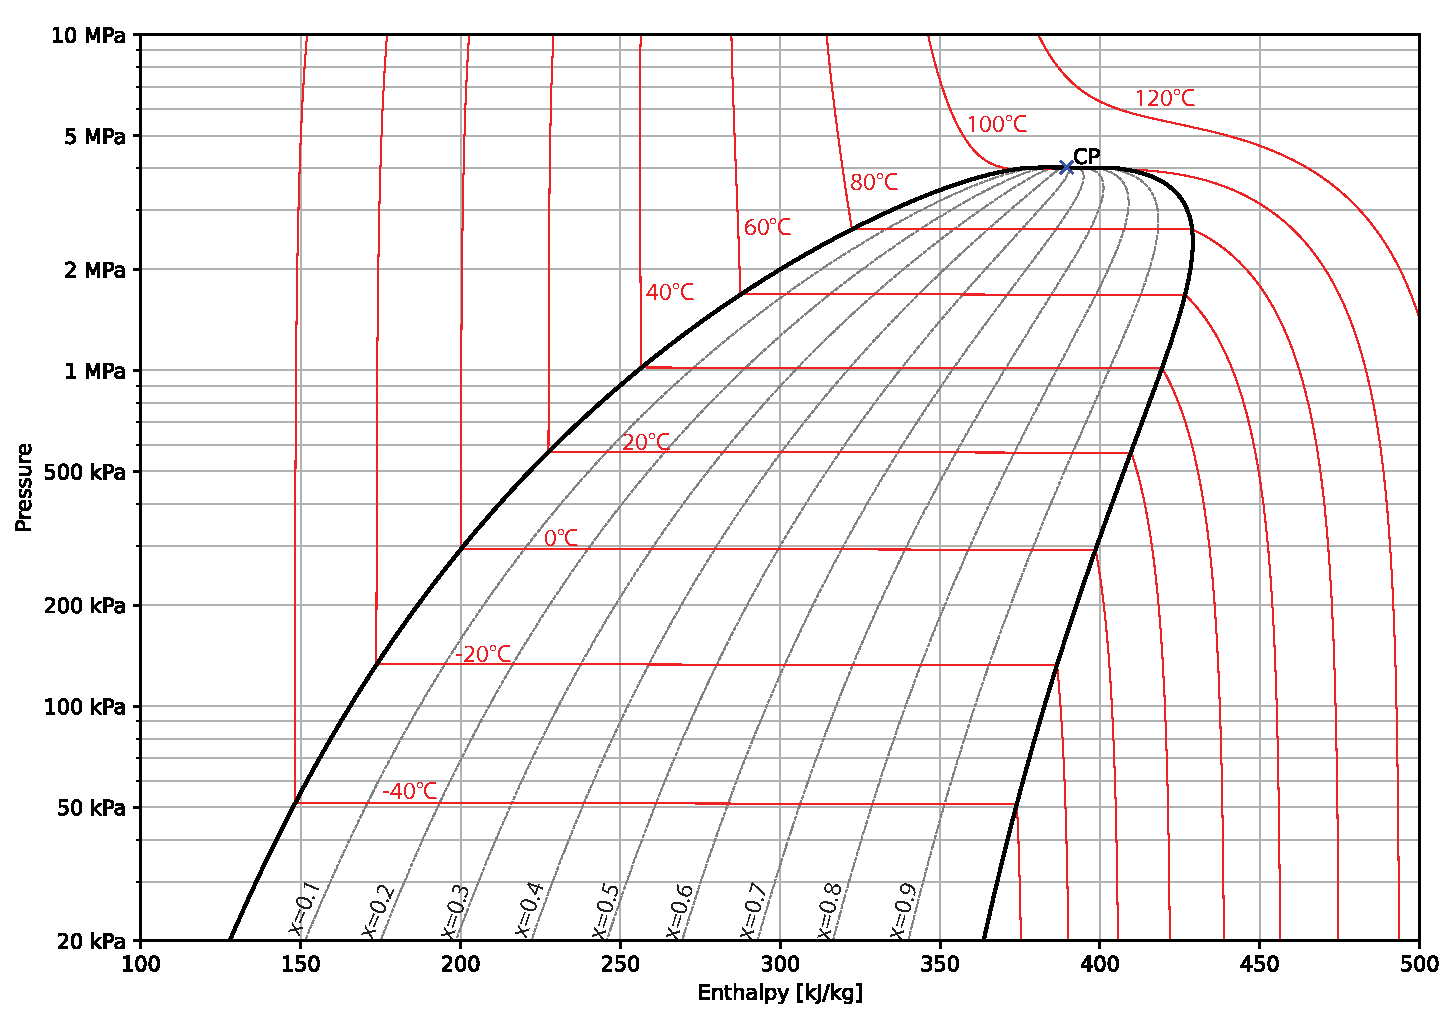
\includegraphics[width=.95\textheight, angle=90]{p-h_R134a}
\end{center}
\section{R134a Enthalpy-Entropy ($h$-$s$) Diagram}
\begin{center}
  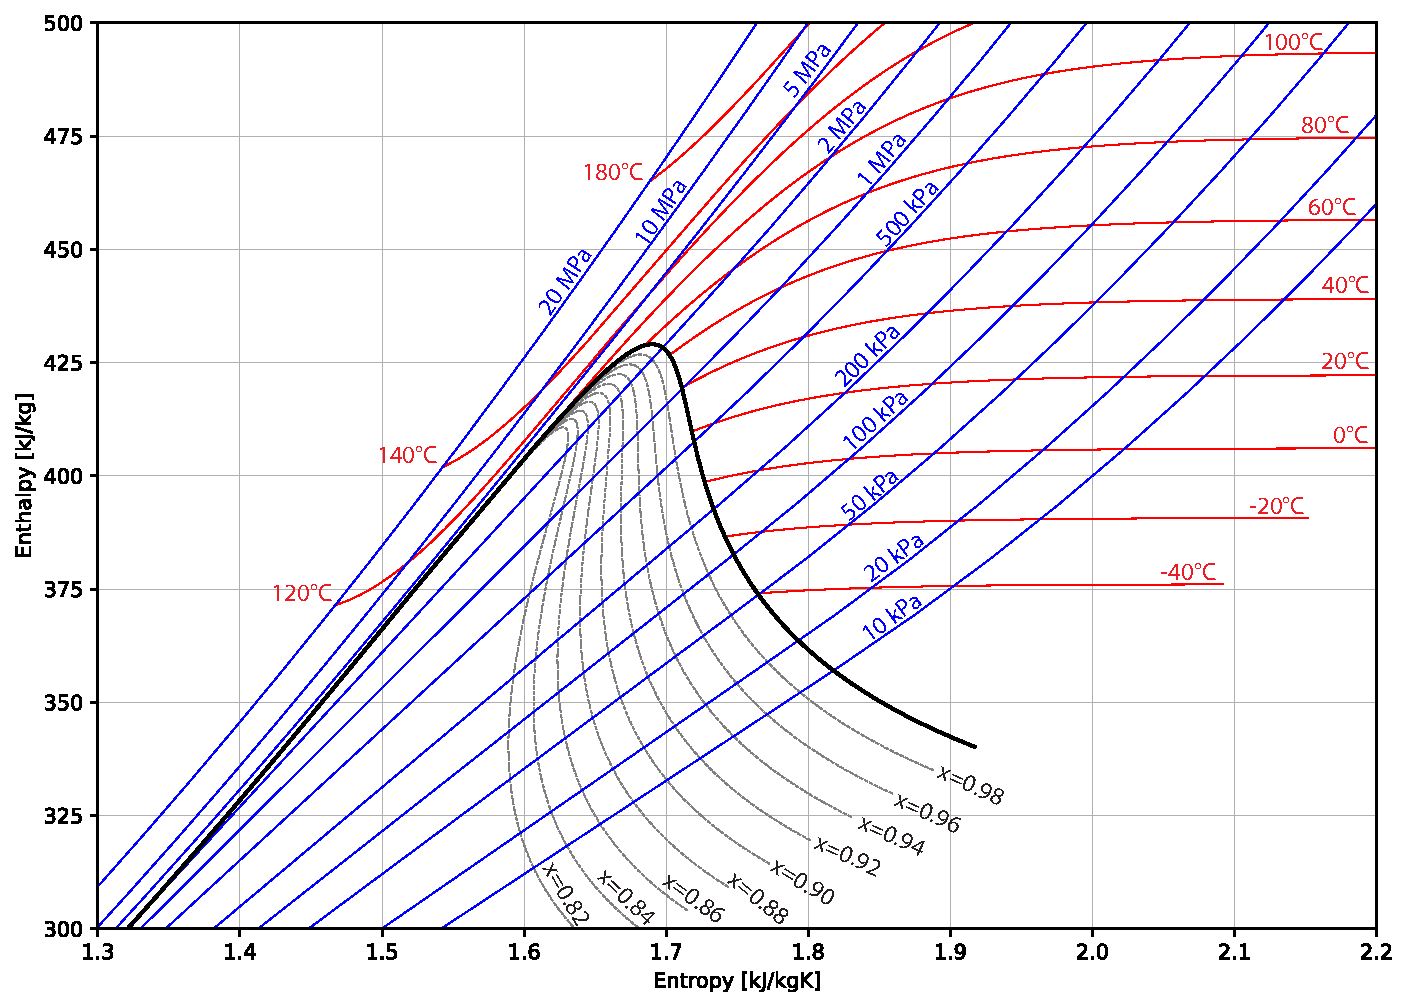
\includegraphics[width=.95\textheight, angle=90]{h-s_R134a}
\end{center}
\restoregeometry

\newgeometry{margin=1.0 in}
\chapter{Properties of Various Ideal Gases}
\section{Properties of Select Ideal Gases at 300 K} \label{sec:idealGasProps}
\resetLTcolor
%\rotatebox{90}{
\begin{longtable}[!ht]{@{\zz\extracolsep{\fill}}c|c|cc|cc|cccc}
  \multicolumn{1}{@{\fullwidthcolor{white}\extracolsep{\fill}}c|}{} &    & \multicolumn{2}{c|}{Gas Constant} & \multicolumn{2}{c|}{Specific Heats} & \multicolumn{4}{c}{Critical Properties} \\
  \multicolumn{1}{@{\fullwidthcolor{white}\extracolsep{\fill}}c|}{Gas Name} & Formula  & $M$ & $R_{gas}$ & $c_v$ & $c_p$ & $T_c$ & $p_c$ & $\rho_c$ & $Z_c$ \\
  \multicolumn{1}{@{\fullwidthcolor{white}\extracolsep{\fill}}c|}{} &          & kg/kmol & kJ/kgK & kJ/kgK & kJ/kgK & K & MPa & kg/$\rm m^3$ & - \\
  \hline\endhead
        Air\footnote[1]{Data from \href{https://pubs.acs.org/doi/10.1021/ie4033999}{CoolProp}} & - & 28.970 & 0.2870 & 0.7177 & 1.0048 & 132.53 & 3.786 & 342.7 & 0.2905 \\ 
        Argon & Ar & 39.948 & 0.2081 & 0.3122 & 0.5203 & 150.69 & 4.863 & 535.6 & 0.2895 \\ 
        Butane & $\rm C_4H_{10}$ & 58.122 & 0.1431 & 1.5594 & 1.7024 & 425.13 & 3.796 & 228.0 & 0.2738 \\ 
        Carbon Dioxide & $\rm CO_2$ & 44.010 & 0.1889 & 0.6569 & 0.8459 & 304.13 & 7.377 & 467.6 & 0.2746 \\ 
        Carbon Monoxide & CO & 28.010 & 0.2968 & 0.7435 & 1.0404 & 132.86 & 3.494 & 303.9 & 0.2915 \\ 
        Ethane & $\rm C_2H_{6}$ & 30.069 & 0.2765 & 1.4760 & 1.7526 &  305.32 & 4.872 & 206.2 & 0.2799 \\ 
        Ethylene & $\rm C_2H_{4}$ & 28.053 & 0.2964 & 1.2393 & 1.5357 &  282.50 & 5.060 & 214.1 & 0.2822 \\ 
        Helium & He & 4.0026 & 2.0773 & 3.1161 & 5.1932 &  5.1953 & 0.228 & 69.58 & 0.3041 \\ 
        Hydrogen & $\rm H_{2}$ & 2.0159 & 4.1245 & 10.186 & 14.310 &  33.145 & 1.296 & 31.26 & 0.3033 \\ 
        Methane & $\rm CH_{4}$ & 16.043 & 0.5183 & 1.7119 & 2.2301 &  190.56 & 4.599 & 162.7 & 0.2863 \\ 
        Neon & Ne & 20.180 & 0.4120 & 0.6181 & 1.0303 &  44.400 & 2.662 & 486.0 & 0.2994 \\ 
        Nitrogen & $\rm N_{2}$ & 28.013 & 0.2968 & 0.7429 & 1.0397 &  126.19 & 3.396 & 313.3 & 0.2894 \\ 
        Octane & $\rm C_8H_{18}$ & 114.23 & 0.0728 & 1.5901 &  1.0458 & 568.74 & 2.484 & 232.0 & 0.2586 \\ 
        Oxygen & $\rm O_{2}$ & 31.999 & 0.2598 & 0.6585 & 0.9183 &  154.58 & 5.043 & 436.1 & 0.2879 \\ 
        Propane & $\rm C_3H_{8}$ & 44.096 & 0.1886 & 1.4828 & 1.6713 &  369.89 & 4.251 & 220.0 & 0.2771 \\ 
        Steam & $\rm H_{2}O$ & 18.015 & 0.4615 & 1.4033 & 1.8649 & 647.10 & 22.064 & 322.0 & 0.2294
\end{longtable}
%}

%% \resetLTcolor
%% %\rotatebox{90}{
%% \begin{longtable}[!ht]{@{\zz\extracolsep{\fill}}c|c|cc|ccccccc}
%%   \multicolumn{1}{@{\fullwidthcolor{white}\extracolsep{\fill}}c}{Gas} & Formula & $M$ & $R_{gas}$ & $c_v$ & $c_p$ & $\gamma$ & $T_c$ & $p_c$ & $\rho_c$ & $Z_c$ \\ \hline\endhead
%%         Air* & - & 28.970 & 0.2870 & 0.7177 & 1.0048 & 1.3999 & 132.53 & 3.786 & 342.7 & 0.2905 \\ 
%%         Argon & Ar & 39.948 & 0.2081 & 0.3122 & 0.5203 & 1.6667 & 150.69 & 4.863 & 535.6 & 0.2895 \\ 
%%         Butane & $\rm C_4H_{10}$ & 58.122 & 0.1431 & 1.5594 & 1.7024 & 1.0917 & 425.13 & 3.796 & 228.0 & 0.2738 \\ 
%%         Carbon Dioxide & $\rm CO_2$ & 44.010 & 0.1889 & 0.6569 & 0.8459 & 1.2876 & 304.13 & 7.377 & 467.6 & 0.2746 \\ 
%%         Carbon Monoxide & CO & 28.010 & 0.2968 & 0.7435 & 1.0404 & 1.3993 & 132.86 & 3.494 & 303.9 & 0.2915 \\ 
%%         Ethane & $\rm C_2H_{6}$ & 30.069 & 0.2765 & 1.4760 & 1.7526 & 1.1874 & 305.32 & 4.872 & 206.2 & 0.2799 \\ 
%%         Ethylene & $\rm C_2H_{4}$ & 28.053 & 0.2964 & 1.2393 & 1.5357 & 1.2392 & 282.50 & 5.060 & 214.1 & 0.2822 \\ 
%%         Helium & He & 4.0026 & 2.0773 & 3.1161 & 5.1932 & 1.6666 & 5.1953 & 0.228 & 69.58 & 0.3041 \\ 
%%         Hydrogen & $\rm H_{2}$ & 2.0159 & 4.1245 & 10.186 & 14.310 & 1.4049 & 33.145 & 1.296 & 31.26 & 0.3033 \\ 
%%         Methane & $\rm CH_{4}$ & 16.043 & 0.5183 & 1.7119 & 2.2301 & 1.3027 & 190.56 & 4.599 & 162.7 & 0.2863 \\ 
%%         Neon & Ne & 20.180 & 0.4120 & 0.6181 & 1.0303 & 1.6668 & 44.400 & 2.662 & 486.0 & 0.2994 \\ 
%%         Nitrogen & $\rm N_{2}$ & 28.013 & 0.2968 & 0.7429 & 1.0397 & 1.3995 & 126.19 & 3.396 & 313.3 & 0.2894 \\ 
%%         Octane & $\rm C_8H_{18}$ & 114.23 & 0.0728 & 1.5901 & 1.6630 & 1.0458 & 568.74 & 2.484 & 232.0 & 0.2586 \\ 
%%         Oxygen & $\rm O_{2}$ & 31.999 & 0.2598 & 0.6585 & 0.9183 & 1.3946 & 154.58 & 5.043 & 436.1 & 0.2879 \\ 
%%         Propane & $\rm C_3H_{8}$ & 44.096 & 0.1886 & 1.4828 & 1.6713 & 1.1271 & 369.89 & 4.251 & 220.0 & 0.2771 \\ 
%%         Steam & $\rm H_{2}O$ & 18.015 & 0.4615 & 1.4033 & 1.8649 & 1.3289 & 647.10 & 22.064 & 322.0 & 0.2294
%% \end{longtable}
%% %}

\section[Ideal Gas Specific Heats of Air]{Ideal Gas Specific Heats of Air\footnotemark[1]} \label{sec:idealGasAir}
\begin{longtable}[!ht]{@{\zz\extracolsep{\fill}}c|cccc||c|cccc}
  \multicolumn{1}{@{\fullwidthcolor{white}\extracolsep{\fill}}c|}{Temp.} & $h$ & $c_v$ & $c_p$ & $\gamma$ & Temp. & $h$ & $c_v$ & $c_p$ & $\gamma$ \\
  \multicolumn{1}{@{\fullwidthcolor{white}\extracolsep{\fill}}c|}{K} & kJ/kg & kJ/kgK & kJ/kgK & - & K & kJ/kg & kJ/kgK &kJ/kgK  & -\\\hline
200 & 326.20 & 0.7154 & 1.0024 & 1.4013 &  1100 & 1287.46 & 0.8717 & 1.1587 & 1.3293 \\
300 & 426.53 & 0.7177 & 1.0048 & 1.3999 &  1150 & 1345.60 & 0.8798 & 1.1668 & 1.3263 \\
400 & 527.37 & 0.7263 & 1.0133 & 1.3952 &  1200 & 1404.14 & 0.8874 & 1.1744 & 1.3235 \\
500 & 629.45 & 0.7423 & 1.0294 & 1.3867 &  1250 & 1463.04 & 0.8945 & 1.1815 & 1.3209 \\
600 & 733.43 & 0.7638 & 1.0509 & 1.3758 &  1300 & 1522.28 & 0.9011 & 1.1882 & 1.3185 \\
700 & 839.70 & 0.7877 & 1.0747 & 1.3644 &  1350 & 1581.85 & 0.9074 & 1.1944 & 1.3163 \\
800 & 948.37 & 0.8115 & 1.0985 & 1.3537 &  1400 & 1641.72 & 0.9132 & 1.2003 & 1.3143 \\
900 & 1059.36 & 0.8337 & 1.1208 & 1.3443 & 1450 & 1701.87 & 0.9188 & 1.2058 & 1.3124 \\
1000 & 1172.46 & 0.8539 & 1.1409 & 1.3362 &1500 & 1762.29 & 0.9239 & 1.2110 & 1.3107 
\end{longtable}



\section[International Standard Atmosphere]{International Standard Atmosphere\footnote[2]{Data from \href{https://pypi.org/project/ambiance/}{ambiance}.}} \label{app:ISA}
\begin{longtable}[!ht]{@{\zz\extracolsep{\fill}}c|cc||c|cc||c|cc}
  \multicolumn{1}{@{\fullwidthcolor{white}\extracolsep{\fill}}c|}{Altitude} & $p$ & $T$ & Altitude & $p$ & $T$ & Altitude & $p$ & $T$\\
  \multicolumn{1}{@{\fullwidthcolor{white}\extracolsep{\fill}}c|}{m} & kPa & K & m & kPa & K & m & kPa & K \\\hline
0.0  & 101.33 & 288.2 & 13.5 & 15.33 & 216.7 & 34 & 0.6634 & 233.7 \\
0.5  & 95.46  & 284.9 & 14.0 & 14.17 & 216.7 & 35 & 0.5746 & 236.5 \\
1.0  & 89.88  & 281.7 & 14.5 & 13.10 & 216.7 & 36 & 0.4985 & 239.3 \\
1.5  & 84.56  & 278.4 & 15.0 & 12.11 & 216.7 & 37 & 0.4332 & 242.1 \\
2.0  & 79.50  & 275.2 & 15.5 & 11.20 & 216.7 & 38 & 0.3771 & 244.8 \\
2.5  & 74.69  & 271.9 & 16.0 & 10.35 & 216.7 & 39 & 0.3288 & 247.6 \\
3.0  & 70.12  & 268.7 & 16.5 & 9.572 & 216.7 & 40 & 0.2871 & 250.3 \\
3.5  & 65.78  & 265.4 & 17.0 & 8.850 & 216.7 & 41 & 0.2511 & 253.1 \\
4.0  & 61.66  & 262.2 & 17.5 & 8.182 & 216.7 & 42 & 0.2200 & 255.9 \\
4.5  & 57.75  & 258.9 & 18.0 & 7.565 & 216.7 & 43 & 0.1930 & 258.6 \\
5.0  & 54.05  & 255.7 & 18.5 & 6.995 & 216.7 & 44 & 0.1695 & 261.4 \\
5.5  & 50.54  & 252.4 & 19.0 & 6.467 & 216.7 & 45 & 0.1491 & 264.2 \\
6.0  & 47.22  & 249.2 & 19.5 & 5.980 & 216.7 & 46 & 0.1313 & 266.9 \\
6.5  & 44.08  & 245.9 & 20.0 & 5.529 & 216.7 & 47 & 0.1159 & 269.7 \\
7.0  & 41.11  & 242.7 & 21.0 & 4.729 & 217.6 & 48 & 0.1023 & 270.7 \\
7.5  & 38.30  & 239.5 & 22.0 & 4.047 & 218.6 & 49 & 0.0903 & 270.7 \\
8.0  & 35.65  & 236.2 & 23.0 & 3.467 & 219.6 & 50 & 0.0798 & 270.7 \\
8.5  & 33.15  & 233.0 & 24.0 & 2.972 & 220.6 & 51 & 0.0705 & 270.7 \\
9.0  & 30.80  & 229.7 & 25.0 & 2.549 & 221.6 & 52 & 0.0622 & 269.0 \\
9.5  & 28.58  & 226.5 & 26.0 & 2.188 & 222.5 & 53 & 0.0549 & 266.3 \\
10.0 & 26.50  & 223.3 & 27.0 & 1.880 & 223.5 & 54 & 0.0483 & 263.5 \\
10.5 & 24.54  & 220.0 & 28.0 & 1.616 & 224.5 & 55 & 0.0425 & 260.8 \\
11.0 & 22.70  & 216.8 & 29.0 & 1.390 & 225.5 & 56 & 0.0374 & 258.0 \\
11.5 & 20.98  & 216.7 & 30.0 & 1.197 & 226.5 & 57 & 0.0328 & 255.3 \\
12.0 & 19.40  & 216.7 & 31.0 & 1.031 & 227.5 & 58 & 0.0287 & 252.5 \\
12.5 & 17.93  & 216.7 & 32.0 & 0.889 & 228.5 & 59 & 0.0251 & 249.8 \\
13.0 & 16.58  & 216.7 & 33.0 & 0.767 & 231.0 & 60 & 0.0220 & 247.0
\end{longtable}


\restoregeometry

\newgeometry{margin=0.5 in}
\section{Compressibility Charts}
\begin{center}
  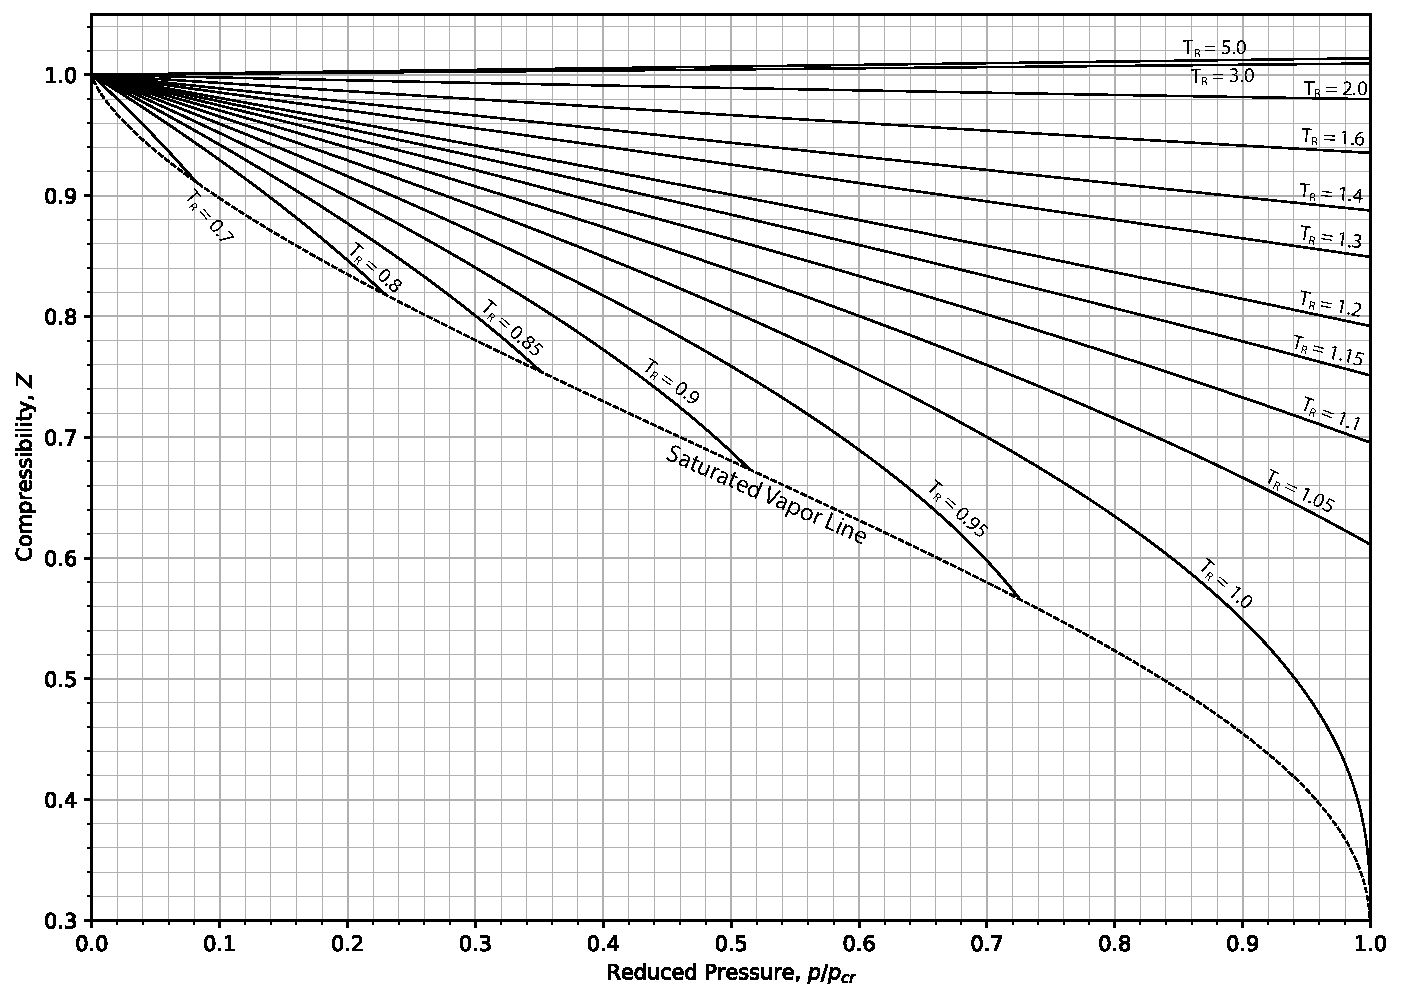
\includegraphics[width=.95\textheight, angle=90]{compressibility-small}
\end{center}
\begin{center}
  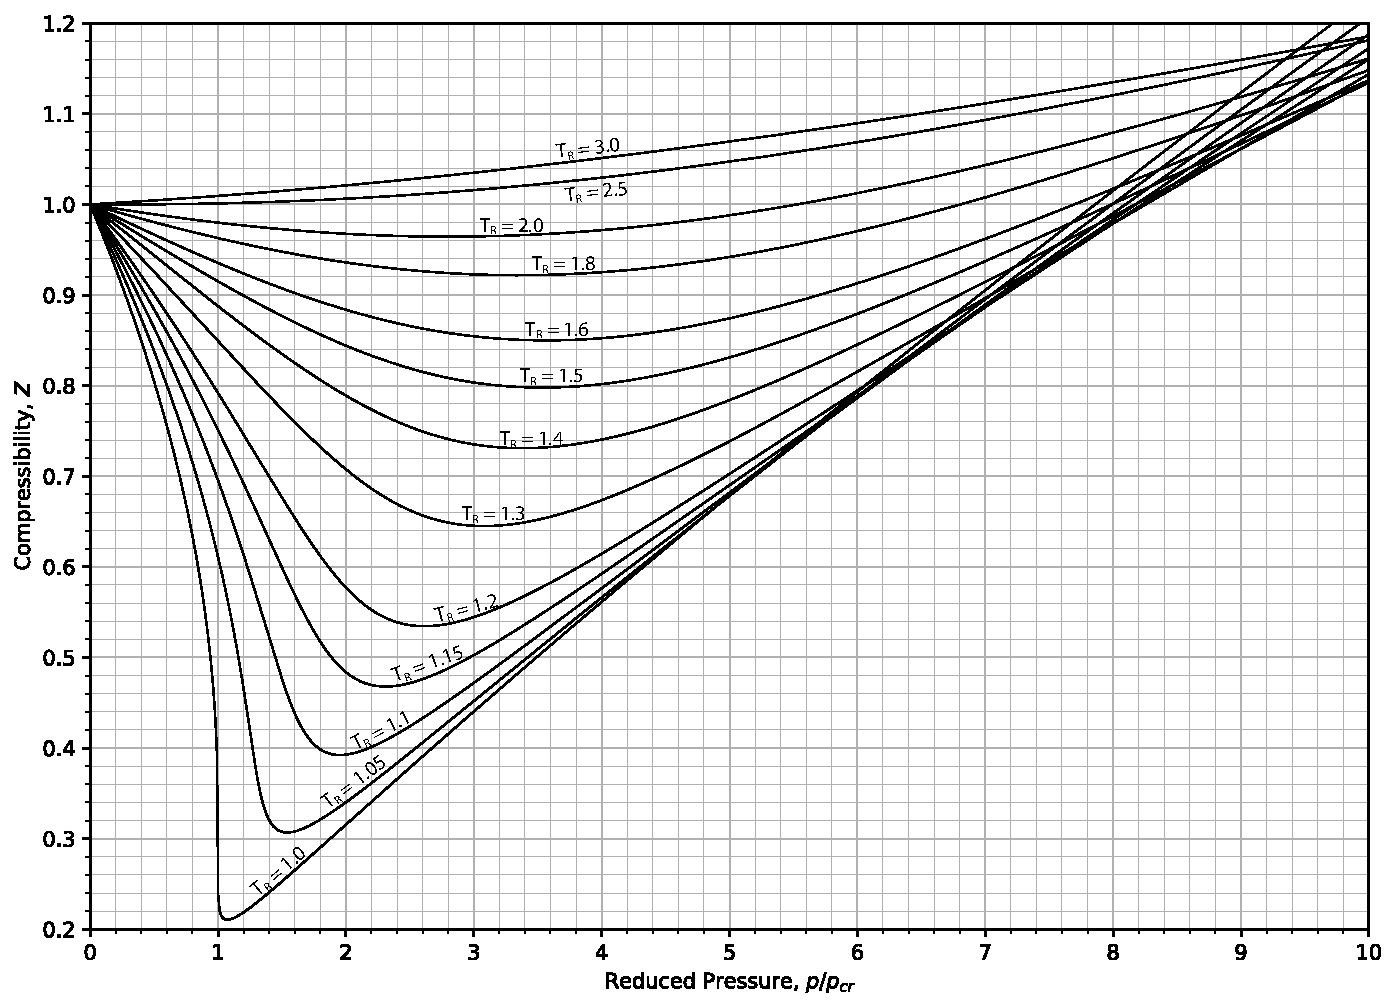
\includegraphics[width=.95\textheight, angle=90]{compressibility-med}
\end{center}
%\section{Critical Properties of Phase-Change Fluids}
\restoregeometry

%\chapter{Psychrometric Chart}

